\documentclass[10pt,compress]{beamer}
\usepackage[ruled,lined,linesnumbered,noend]{algorithm2e}
%\usepackage[chapter,ruled,rightnl,lined,vlined]{algorithm}
%\usepackage[noend]{algorithmic}
%\floatname{algorithm}{Algoritmo}
\renewcommand{\listalgorithmname}{Lista de algoritmos}
\renewcommand{\algorithmicrequire}{\textbf{Entrada:}}
\renewcommand{\algorithmicensure}{\textbf{Salida:}}
%\renewcommand{\algorithmicecomment}{\textbf{//}}
\renewcommand{\algorithmicend}{\textbf{Fin}}
\renewcommand{\algorithmicif}{\textbf{Si}}
\renewcommand{\algorithmicthen}{\textbf{Entonces}}
\renewcommand{\algorithmicelse}{\textbf{Sino}}
\renewcommand{\algorithmicelsif}{\algorithmicelse,\ \algorithmicif}
\renewcommand{\algorithmicendif}{\algorithmicend\ \algorithmicif}
\renewcommand{\algorithmicfor}{\textbf{Para}}
\renewcommand{\algorithmicforall}{\textbf{Para todo}}
\renewcommand{\algorithmicdo}{\textbf{Hacer}}
\renewcommand{\algorithmicendfor}{\algorithmicend\ \algorithmicfor}
\renewcommand{\algorithmicwhile}{\textbf{Mientras}}
\renewcommand{\algorithmicendwhile}{\algorithmicend\ \algorithmicwhile}
\renewcommand{\algorithmicloop}{\textbf{Repetir}}
\renewcommand{\algorithmicendloop}{\algorithmicend\ \algorithmicloop}
\renewcommand{\algorithmicrepeat}{\textbf{Repetir}}
\renewcommand{\algorithmicuntil}{\textbf{Hasta que}}
\renewcommand{\algorithmicprint}{\textbf{Imprimir}} 
\renewcommand{\algorithmicreturn}{\textbf{Retornar}} 
\renewcommand{\algorithmictrue}{\textbf{Cierto }} 
\renewcommand{\algorithmicfalse}{\textbf{Falso }} 
 % mi archivo de traduccion
\usepackage{graphicx}
\usepackage[spanish]{babel}
\usepackage{amsmath,amssymb}
\usepackage{colortbl}
%\usepackage[francais]{babel}
\usepackage[spanish]{layout}
\usepackage[utf8x]{inputenc}
\usepackage{nantes_theme}
\usepackage{epsfig}
\setbeamercolor{background canvas}{bg=white}
\usepackage{marvosym}
\usepackage{wasysym}
%\justifying
% -- Colors used ---------------------------------------------------------
\usepackage{fancybox}
%\usepackage{slidesec}
%\usepackage{latexsym}
%\usepackage{graphicx}
%\usepackage{amssymb}
%\usepackage{amsmath}
% \usepackage{graphicx}
% \usepackage{rotate}
% \usepackage{lscape}
% \usepackage{xspace}
% \usepackage{float}
% \usepackage{color}
 
%\definecolor{vertfonce} {rgb}{0.03,0.345,0.427}
%\definecolor{mauvefonce} {rgb}{0.5,0.0,0.5}
%\definecolor{vertMIC} {rgb}{0.51,0.76,0.15}

\newcommand{\BLEU}[1]{\textcolor{blue}{{\bf #1}}\xspace}
%\newcommand{\PINK}[1]{\textcolor{magenta}{{\bf #1}}\xspace}
%\newcommand{\ROUGE}[1]{\textcolor{red}{{\bf #1}}\xspace}
%\newcommand{\FLUO}[1]{\colorbox{yellow}{#1}\xspace}
%\newcommand{\CYAN}[1]{\colorbox{cyan}{#1}\xspace}
%\newcommand{\MAUVEn}[1]{\textcolor{mauvefonce}{ #1}\xspace}
%\newcommand{\VERTMIC}[1]{\textcolor{vertMIC}{{\bf #1}}\xspace}

%%\definecolor{tbon} {rgb}{0.000,1.000,0.000}
%\newrgbcolor{tbon} {0.000 1.000 0.000}
%\newrgbcolor{abon} {0.500 0.900 0.000}
%\newrgbcolor{bof} {0.900 0.600 0.000}
%\newrgbcolor{tnul} {1.000 0.000 0.000}
%
%\newrgbcolor{lightblue} {0.000 0.000 0.500}
%
%\newcommand{\TBON}[1]{\colorbox{tbon}{#1}\xspace}
%\newcommand{\ABON}[1]{\colorbox{abon}{#1}\xspace}
%\newcommand{\BOF}[1]{\colorbox{bof}{#1}\xspace}
%\newcommand{\TNUL}[1]{\colorbox{tnul}{#1}\xspace}

\renewcommand*{\algorithmcfname}{Algoritmo}

\definecolor{VERTC} {rgb}{0.81,0.99,0.78}
\definecolor{VERTM} {rgb}{0.41,0.99,0.41}
\definecolor{VERTF} {rgb}{0.16,0.99,0.03}
\newcommand{\BOXVERTC}[1]{\colorbox{VERTC}{#1}\xspace}
\newcommand{\BOXVERTM}[1]{\colorbox{VERTM}{#1}\xspace}
\newcommand{\BOXVERTF}[1]{\colorbox{VERTF}{#1}\xspace}

\definecolor{ROUGEC} {rgb}{0.99,0.78,0.78}
\definecolor{ROUGEM} {rgb}{0.99,0.41,0.41}
\definecolor{ROUGEF} {rgb}{0.99,0.03,0.03}
\newcommand{\BOXROUGEC}[1]{\colorbox{ROUGEC}{#1}\xspace}
\newcommand{\BOXROUGEM}[1]{\colorbox{ROUGEM}{#1}\xspace}
\newcommand{\BOXROUGEF}[1]{\colorbox{ROUGEF}{#1}\xspace}


\title{Uso de un Algoritmo de C\'umulo de Part\'iculas \\ 
       Basado en Hipervolumen para \\ Resolver Problemas Multi-Objetivo}
%\subtitle{\subtitle}
\author[MOPSOhv]{
		\vspace{2mm}\\{\textbf{Ing. Iv\'an Christhofer Chaman Garc\'ia}} \\
			Asesor:\\
		\textbf{Dr. Carlos A. Coello Coello}
}
\institute{
\begin{center}
\textbf{
Centro de Investigaci\'on y de Estudios Avanzados \\
del Instituto Polit\'ecnico Nacional \\
Departamiento de Computaci\'on. \\}
\end{center}
}
\date{\footnotesize{\vspace{2mm}\\
\textbf{5 de Octubre de 2012}}}
\beamertemplatetransparentcovered

\setbeamercolor{frametitle}{bg=lightgray}

\begin{document}

%
% =========================================================================================================
%
{ % Redefinition du bas du style afin de ne pas afficher le numero de slide sur la page 1
  \defbeamertemplate*{footline}{}
  {
    \leavevmode%
    \hbox{%
    \begin{beamercolorbox}[wd=.25\paperwidth,ht=2.25ex,dp=1ex,left]{authors in head/foot}%
        \usebeamerfont{author in head/foot}\hspace*{1ex}
     \end{beamercolorbox}%
    \begin{beamercolorbox}[wd=.75\paperwidth,ht=2.25ex,dp=1ex,right]{authors in head/foot}%
        \usebeamerfont{author in head/foot}\insertshortauthor\hspace*{1ex}
    \end{beamercolorbox}}%
    \vskip0pt%
}

	\frame{\titlepage}
}
% =========================================================================================================
\section{Introducci\'on}
\frame{\tableofcontents[currentsection]}
\begin{frame}
\frametitle{Motivaci\'on}

El uso de esquemas de selecci\'on basados en la dominancia de Pareto presenta diversas limitantes, dentro de las que destaca
su pobre escalabilidad cuando se aumenta la cantidad de funciones objetivo. Una de las alternativas m\'as prometedoras es el uso 
de indicadores de desempe\~no para seleccionar soluciones.

	\begin{block}{Principales objetivos de este trabajo}
	\begin{itemize}
	%\justifying
	\item Implementar un algoritmo basado en c\'umulos de particulas para resolver problemas multi-objetivo que use el hipervolumen 
	para seleccionar a los mejores l\'ideres que conducir\'an la b\'usqueda.
	\item El nuevo algoritmo deber\'a ser competitivo con respecto a algoritmos evolutivos multi-objetivo del estado del arte.
	\item Comparar el desempe\~no del algoritmo propuesto utilizando un conjunto diverso de problemas de la literatura especializada.	
	\end{itemize}
	\end{block}
\end{frame}
% =========================================================================================================
\subsection{Optimizaci\'on multi-objetivo}
    \begin{frame}
		\frametitle{Modelando un problema de optimizaci\'on multi-objetivo}
		\[
		\left[\begin{array}{ccc}
			opt & f_i(\vec{x}) & \forall i \in \{1,...,k\} \\
			con &  & \\
				& g_j(\vec{x}) \leq 0 & \forall j \in \{1,...,i\} \\
				& h_k(\vec{x}) = 0 & \forall k \in \{1,...,j\} \\
				& x_l \in [l_b, u_b] & \forall l \in \{1,...,n\} \\
		\end{array}\right]
		\]
    \begin{block}{donde:}
	  \begin{itemize}
		%\justifying
			\item $opt \in \{\min, \max\}$,
			\item $k$ es el n\'umero de funciones objetivo,
			\item $i$ es el n\'umero de restricciones de desigualdad,
			\item $j$ es el n\'umero de restricciones de igualdad,
			\item $n$ es el n\'umero de variables de decisi\'on del problema,
			\item $l_b, u_b$ son los intervalos del problema (inferior y superior, respectivamente) de cada variable $x_l$.
	  \end{itemize}
	\end{block}
	En adelante,  supondremos s\'olo problemas de minimizaci\'on.
\end{frame}
% =========================================================================================================
\begin{frame}
	\frametitle{Ejemplo de un problema con dos objetivos}	
		\begin{figure}[h!]
			\centering
				\includegraphics[scale=0.4]{ejemplo.eps}
				
     \end{figure}
\end{frame}
% =========================================================================================================
  \subsection{Definiciones}
	
\begin{frame}
	\frametitle{Definiciones y notaciones}
	\begin{block}{Dominancia de Pareto}
	Un vector $\vec{u} = \left(u_1, \ldots, u_k \right)$ se dice que domina a $\vec{v} = \left(v_1, \ldots, v_k \right)$,
	  denotado por $\vec{u} \preceq \vec{v}$, si y s\'olo si $\vec{u}$ es parcialmente menor que $\vec{v}$, es decir, 
	  $\forall i \in \left\{1, \ldots, k \right\}: u_i \leq v_i \wedge \exists i \in \left\{1, \ldots, k\right\}: u_i < v_i$.
	\end{block}
		\begin{figure}[h!]
			\centering
				\includegraphics[scale=0.4]{dominancia.eps}
			
     \end{figure}	
\end{frame}
% =========================================================================================================
\begin{frame}
	\frametitle{Definiciones y notaciones}	
	\begin{block}{Conjunto de \'optimos de Pareto}
	Los elementos del conjunto de \'optimos de Pareto tienen vectores objetivo que no pueden ser mejorados sin empeorar al menos otro
  objetivo. Los vectores objetivo de las soluciones \'optimas de Pareto se denominan vectores \textit{no dominados}. 	
	\end{block}
\end{frame}
% =========================================================================================================
\begin{frame}
	\frametitle{Definiciones y notaciones}
	\begin{block}{Frente de Pareto} 
	Los vectores de las funciones objetivo correspondientes al conjunto de \'optimos de Pareto conforman el denominado frente de Pareto  	
	\end{block}
	
	\begin{figure}[h!]
			\centering
				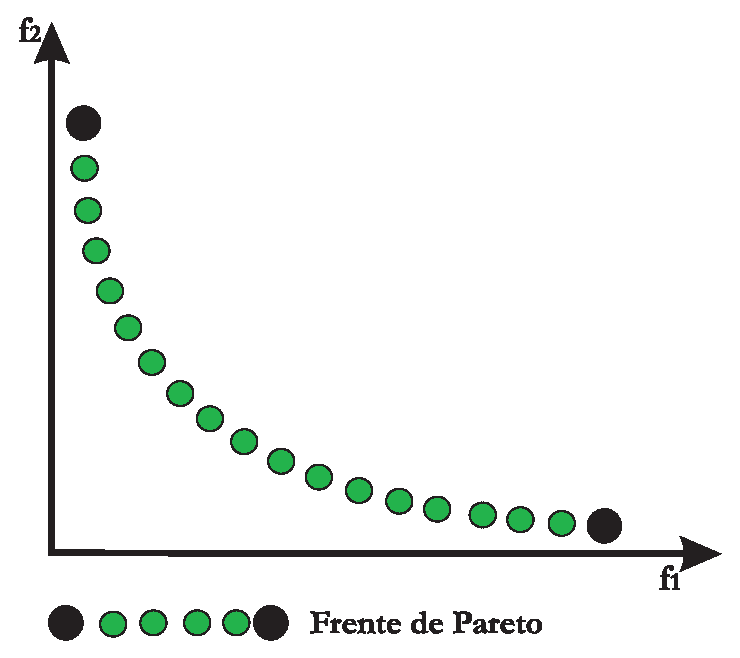
\includegraphics[scale=0.4]{frenteP.eps}
				
     \end{figure}	
\end{frame}
% =========================================================================================================
\begin{frame}
	\frametitle{Definiciones y notaciones}		
	\begin{block}{Vector ideal y vector de Nadir}
	 \[  f_{ideal}= \left(^{\min}_{\vec{x}\in P^*}f_1\left(\vec{x}\right), \ldots, ^{\min}_{\vec{x}\in P^*}f_k\left(\vec{x}\right) \right)\]
\[  f_{nadir}= \left(^{\max}_{\vec{x}\in P^*}f_1\left(\vec{x}\right), \ldots, ^{\max}_{\vec{x}\in P^*}f_k\left(\vec{x}\right) \right)\]
	\end{block}
	
	\begin{figure}[h!]
			\centering
				\includegraphics[scale=0.4]{idealnadir.eps}	
							
     \end{figure}	
\end{frame}

% =========================================================================================================
\begin{frame}
	\frametitle{Objetivos de la optimizaci\'on multi-objetivo}
	El objetivo principal de la optimizaci\'on multi-objetivo es generar el mayor n\'umero posible de elementos del conjunto de \'optimos de Pareto.
	
	\begin{block}{Convergencia}
		Permite medir hasta qu\'e punto las soluciones encontradas pertencen al verdadero frente de Pareto.
	\end{block}
	\begin{block}{Espaciado}
		Indica qu\'e tan bien distribuidas est\'an las soluciones en el verdadero frente de Pareto (o su aproximaci\'on).
	\end{block}
	Al solocuionar un problema multi-objetivo se busca llegar lo m\'as r\'apido posible al verdadero frente de Pareto (convergencia), 
	produciendo un conjunto bien distribuido de soluciones a lo largo del frente de Pareto (Espaciado).
\end{frame}

% =========================================================================================================
\subsection{Algoritmos evolutivos}

\begin{frame}
\frametitle{¿Por qu\'e algoritmos evolutivos?}
Un algoritmo evolutivo utiliza algunos mecanismos inspirados en la evoluci\'on biol\'ogica, que han demostrado ser eficaces en un gran conjunto de problemas dif\'iciles. 
\'Estos est\'an basados ​​en una poblaci\'on, ya que utilizan un conjunto (poblaci\'on) de soluciones que se actualizan en cada iteraci\'on (generaci\'on).
	\begin{block}{Caracter\'isticas}
	  \begin{itemize}
			\item No requieren de conocimientos espec\'ificos sobre el problema.
			\item Pueden actuar como eficaces optimizadores globales, ya que son menos propensos a quedar atrapados en 
						\'optimos locales.
			\item Son f\'aciles de comprender e implementar en forma secuencial y paralela.
			\item Se pueden hibridar con otras t\'ecnicas de optimizaci\'on (por ejemplo, t\'ecnicas de programaci\'on 
						matem\'atica).
	  \end{itemize}
	\end{block}
\end{frame}
% =========================================================================================================
\begin{frame}
	\frametitle{Elitismo}	
	\begin{block}{Implementaci\'on del elitismo }
		\begin{itemize}
   \item Combinar la poblaci\'on anterior y la nueva.
   \item Mantener una poblaci\'on secundaria llamada archivo hist\'orico.   
  \end{itemize}
  \end{block}
	
	  \begin{figure}[H]
	\centering
	\includegraphics[scale=0.40]{elitismo.eps}
     
      \end{figure}
	
\end{frame}
% =========================================================================================================
\subsection{Optimizaci\'on por c\'umulo de part\'iculas}
\begin{frame}
	\frametitle{C\'umulos de Part\'iculas}
Un algoritmo de optimizaci\'on basado en c\'umulos de part\'iculas o \textit{Particle Swarm Optimization (PSO)} es una t\'ecnica inspirada en el 
  comportamiento social del vuelo de las aves o el movimiento de los bancos de peces que intentan encontrar comida.
	
	\begin{block}{Principales caracter\'isticas}
	    \begin{itemize}
   \item La poblaci\'on es inicializada aleatoriamente y evoluciona iterativamente buscando la mejor soluci\'on posible.
   \item Realiza una b\'usqueda ciega.
   \item Trabaja con informaci\'on codificada (binaria, entera o real).
   \item Es una t\'ecnica de b\'usqueda estoc\'astica.
  \end{itemize}
	\end{block}
	
	\begin{block}{Direcci\'on de b\'usqueda}  
  \begin{itemize}
   \item Su conocimiento sobre el entorno. 
   \item Su conocimiento hist\'orico.
   \item La estructura de su vecindario.
  \end{itemize} 
	\end{block}
\end{frame}
% =========================================================================================================

\begin{frame}
	\frametitle{Estructura y trayectoria de una part\'icula}
	 \begin{figure}
	\centering
	\includegraphics[scale=0.50]{trayectoria.eps}
     
      \end{figure}						
\end{frame}

% =========================================================================================================
\begin{frame}
	\frametitle{El coraz\'on de esta heur\'istica}
	\begin{block}{Cambiar la velocidad}
	\[
	  \vec{v}^{t+1}_{i} \leftarrow \vec{v}^t_i + \phi_1 \cdot rnd_1 \cdot \left(\vec{pBest}^t_i - \vec{x}^t_i \right) 
					    + \phi_2 \cdot rnd_2 \cdot \left(\vec{g}^t - \vec{x}^t_i \right) 
    \]	
		\end{block}
	\begin{block}{Cambiar la posici\'on}
		\[
	  \vec{x}^{t+1}_i \leftarrow  \vec{x}^t_i + \vec{v}^t_i
      \]
  \end{block}
\end{frame}
% =========================================================================================================
\begin{frame}
	\frametitle{Algoritmo can\'onico}
	   \begin{algorithm}[H]
				Funci\'on a optimizarse $f\left(\vec{x}\right)$\;	
				Iniciar el contador de generaci\'on es $t=0$\;
				Iniciar aleatoriamente $\vec{x}^0$ y $\vec{v}^0$ de todo el C\'umulo \;
				Evaluar la funci\'on objetivo con las posiciones $\vec{x}^{0}$\;
				Encontrar $\vec{pBest}^0$\;
				Encontrar $\vec{g}^0$\;
				\While{$t < maxG$}{
					\For{ $\forall i$ part\'iculas del C\'umulo}{
						$\vec{v}^{t+1}_{i}\leftarrow \vec{v}^{t}_{i}+\phi_{1}\cdot rnd_{1} \cdot \left(\vec{pBest}^{t}-x^{t}_{i}\right)+\phi_{2}\cdot rnd_{2} \cdot \left(\vec{g}^{t}-\vec{x}^{t}_{i}\right)$\;
						$\vec{x}^{t+1}_{i} \leftarrow \vec{x}^{t}_{i}+\vec{v}^{t+1}_{i}$\;
						Evaluar la funci\'on objetivo con las nuevas posiciones $\vec{x}^{t+1}$\;
				}
				Encontrar $\vec{pBest}^t$\;
				Encontrar $\vec{g}^t$\;
				$t=t+1$\;				
			}
			\Return La mejor soluci\'on encontrada\;
		\caption{PSO can\'onico}
\end{algorithm}
\end{frame}
% =========================================================================================================

\begin{frame}
	\frametitle{Entornos de interacci\'on}
	\begin{figure}
	\centering
	\includegraphics[scale=0.50]{entornos.eps}	  
      
      \end{figure}
\end{frame}
% =========================================================================================================
\begin{frame}
	\frametitle{Topolog\'ias de vecindarios}
 \begin{figure}
	\centering
	\includegraphics[scale=0.40]{vecindarios.eps}	
 
      \end{figure}
\end{frame}
% =========================================================================================================

 \begin{frame}
	\frametitle{Aspectos avanzados del algoritmo}
		\begin{block}{Control de velocidad}
			\[	   
				\vec{v}^t_i = \{
						\begin{matrix} 
								\vec{v}^{t+1}_i & \mbox{si}& \vec{v}^{t+1}_i < \vec{v}_{\max}\\
								\vec{v}_{\max} & \mbox{si}& \vec{v}^{t+1}_i \geq \vec{v}_{\max}
						\end{matrix}    
			\]	
		\end{block}
	\begin{block}{Factor de constricci\'on}
		\[  \vec{v}^{t+1}_{i} = \chi \left( \vec{v}^t_i + \phi_1 \cdot rnd_1 \cdot \left(\vec{pBest}^t_i - \vec{x}^t_i \right) 
					    + \phi_2 \cdot rnd_2 \cdot \left(\vec{g}^t - \vec{x}^t_i \right) \right) 
     \]
  \end{block}
		\begin{block}{Factor de inercia}
		\[  
		\vec{v}^{t+1}_{i} = \omega \cdot \vec{v}^t_i + \phi_1 \cdot rnd_1 \cdot \left(\vec{pBest}^t_i - \vec{x}^k_i \right) 
					    + \phi_2 \cdot rnd_2 \cdot \left(\vec{g}^t - \vec{x}^t_i \right) 
     \]
  \end{block}
\end{frame}
% =========================================================================================================

\begin{frame}
	\frametitle{Modelos de configuraci\'on}
	
	\begin{block}{Modelo completo}
     \textbf{$\phi_1 > 0 \text{ y } \phi_2 > 0$} 
	\end{block}
	\begin{block}{Modelo cognitivo}
     \textbf{$\phi_1 > 0 \text{ y } \phi_2 = 0$} 
	\end{block}
	\begin{block}{Modelo social}
     \textbf{$\phi_1 = 0 \text{ y } \phi_2 > 0$}
	\end{block}
	\begin{block}{Modelo social exclusivo}
     \textbf{$\phi_1 = 0 \text{, } \phi_2 > 0 \text{ y } \vec{g} \neq \vec{x}_i$}
  \end{block}
\end{frame}
% =========================================================================================================

\begin{frame}
	\frametitle{Descripci\'on de la versi\'on multi-objetivo}	
	\begin{block}{Dificultad}
			No existe una noci\'on clara de c\'omo seleccionar mejor los lideres de cada part\'icula hasta el momento o de un vecindario.
  \end{block}
	
	\begin{block}{Metas principales}
		\begin{itemize}
   \item Maximizar el mayor n\'umero de elementos del conjunto de \'optimos de Pareto.
   \item Minimizar la distancia entre las soluciones obtenidas por el algoritmo y el conjunto de \'optimos de Pareto.
   \item Maximizar la dispersi\'on de las soluciones encontradas, de modo que podamos tener una distribuci\'on lo m\'as uniforme posible.	
  \end{itemize}
  \end{block}
\end{frame}
% =========================================================================================================

\begin{frame}
	\frametitle{Algoritmo can\'onico multi-objetivo}
	   \begin{algorithm}[H]
				Problema de optimizaci\'on multi-objetivo $F\left(\vec{x}\right)$\;	
				Iniciar aleatoriamente $\vec{x}^0$ y $\vec{v}^0$ de todo el C\'umulo\;							
				Evaluar las funciones objetivo con las part\'iculas del C\'umulo\;
				Seleccionar el $\vec{pBest}^0$ inicial de las part\'iculas\;
				Insertar las part\'iculas no dominadas en el archivo $A^{0}$\;
				\While{$t < maxG$}{
					Seleccionar un $g^t$\;					
					\For{ $\forall i$ part\'iculas del C\'umulo }{
							$\vec{v}^{t+1}_{i}\leftarrow\omega\cdot \vec{v}^{t}_{i}+\phi_{1}\cdot rnd_{1} \cdot \left(\vec{pBest}^{t}_{i}-\vec{x}^{k}_{i}\right) +\phi_{2}\cdot rnd_{2} \cdot \left(\vec{g}^{t}-\vec{x}^{k}_{i}\right)$\;
							$\vec{x}^{t+1}_{i}\leftarrow \vec{x}^{t}_{i}+\vec{v}^{t+1}_{i}$\;
			    }					
					Evaluar las funciones objetivo con las part\'iculas del C\'umulo\;
					Actualizar el $\vec{pBest}^t$ de las part\'iculas\;
					Actualizar las part\'iculas no dominadas en el archivo $A^{t}$\;
					$t\leftarrow t+1$\;
	}
	\Return Soluciones no dominadas en un archivo $A$\;
		\caption{PSO can\'onico multi-objetivo}
\end{algorithm}
\end{frame}

% =========================================================================================================

\subsection{Estado del arte}
\begin{frame}
	\frametitle{NSGA-II}
	El NSGA-II es muy popular en la literatura especialzada debido,  sobre todo, a su eficiencia y facilidad de uso.
	\begin{block}{Caracter\'isticas}
		\begin{itemize}
				\item Esta basado en la dominancia de Pareto.
				\item Realiza un ordenamiento no dominado con base base en los niveles o jerarqu\'ias de no dominancia ($rank$).				
				\item No requiere especificar par\'ametros adicionales para la preservaci\'on de la diversidad en la poblaci\'on.				
				\item Se utiliza la distancia de \textit{Crowding} para evaluar la diversidad de las soluciones.
  \end{itemize}
	\end{block}
\end{frame}
% =========================================================================================================

\begin{frame}
	\frametitle{SMS-EMOA}
	El SMS-EMOA es un algoritmo cuyo mecanismo de selecci\'on adopta el hipervolumen.
	\begin{block}{Caracter\'isticas}	
				\begin{itemize}
					\item Genera en cada iteraci\'on nuevas soluciones por medio de operadores de variaci\'on aleatoria
					\item Realiza un ordenamiento no dominado con base en los niveles o jerarqu\'ias de no dominancia ($rank$) igual que el NSGA-II.
					\item El hipervolumen se aplica como criterio de selecci\'on para descartar individuos.
					\item Su principal inconveniente es su alto costo computacional
   \end{itemize}  
	\end{block}
\end{frame}
% =========================================================================================================

\begin{frame}
	\frametitle{MOPSOcd}
	El MOPSOcd incorpora la distancia de \textit{Crowding} para seleccionar al mejor l\'ider global y para mantener las soluciones no dominadas 
  en el archivo externo.
	\begin{block}{Caracter\'isticas}
		\begin{itemize}
			\item Hace uso de un operador de mutaci\'on junto a la distancia de \textit{Crowding}.  
			\item La selecci\'on del mejor l\'ider global se hace de las soluciones no dominadas con los valores m\'as altos de la distancia de \textit{Crowding}. 
			\item Ordenamiento de la poblaci\'on con base en la distancia de \textit{Crowding}.
			\item La selecci\'on de diferentes gu\'ias para cada part\'icula en una parte determinada del archivo.
			\item Los resultados muestran que este algoritmo es competitivo en lo que a 
					convergencia hacia el frente de Pareto se refiere, generando tambi\'en un conjunto bien distribuido de soluciones no dominadas. 
			\item Adopta el mecanismo para el manejo de restricciones usado por el NSGA-II.
  \end{itemize}  
 
	\end{block}
\end{frame}
% =========================================================================================================

\subsection{Hipervolumen}
\begin{frame}
	\frametitle{Hipervolumen}
	 El hipervolumen es un indicador muy com\'un que se utiliza para medir y comparar la calidad de las soluciones
  finales producidas por un algoritmo evolutivo.
	
	\begin{block}{Definici\'on}
		El hipervolumen representa la surperficie (o el volumen para m\'as de 2 objetivos) y es ``el tama\~no del espacio cubierto o del espacio dominado''
		por las soluciones encontradas hasta el momento.
	\end{block}  

	\begin{block}{Definici\'on formal}
		Dada $\Lambda$ que denota la m\'etrica de \textit{Lebesgue} 
   o m\'etrica $\mathcal{S}$, el hipervolumen es definido formalmente como:
		\[
		\mathcal{S}(\mathcal{P},y_{ref}) = \Lambda \left(\bigcup_{y \in \mathcal{P}} \left\{ y' |~ y \prec y' \prec y_{ref} \right\} \right), 
		\mathcal{P} \subseteq \mathbb{R}^m
		\]
	\end{block}
\end{frame} 
% =========================================================================================================
\begin{frame}
	\frametitle{Hipervolumen por punto de referencia}
	\begin{figure}
	\centering
	\includegraphics[scale=0.4]{puntoref.eps}
      
      \end{figure}
\end{frame}
% =========================================================================================================

\begin{frame}
	\frametitle{Hipervolumen vs contribuci\'on al hipervolumen}	
	\begin{block}{Indicador de hipervolumen}
		\begin{itemize}
		\item Es el \'unico que garantiza la monotonicidad estricta con respecto a la relaci\'on de dominancia de Pareto.
		\item El c\'alculo del hipervolumen es muy costoso computacionalmente hablando.	
		\item Invariante a la escala.		
		\end{itemize}
	\end{block}
	\begin{block}{Contribuci\'on al hipervolumen}
		\begin{itemize}
		\item S\'olo se considera la contribuci\'on de las soluciones en la maximizaci\'on del hipervolumen.
		\item Complejidad aceptable.
		\item F\'acil implementaci\'on.
		\item La aproximaci\'on elegida puede ser diferente al \'optimo de Pareto.
		\item Tiene un cierto error (aproximadamente $<35 \%$).
		\end{itemize}
	\end{block}
\end{frame}

% =========================================================================================================
\begin{frame}
	\frametitle{Contribuci\'on al hipervolumen}
   \begin{figure}
    \centering
    \includegraphics[scale=0.5]{contribucion.eps}
    
    \end{figure}
\end{frame}
% =========================================================================================================
\begin{frame}
	\frametitle{Elecci\'on del punto de referencia}
	   \begin{figure}
	\centering
	\includegraphics[scale=0.4]{eleccionref.eps}	  
      
      \end{figure}
\end{frame}
% =========================================================================================================

\section{Algoritmo MOPSOhv}
\frame{\tableofcontents[currentsection]}
\subsection{Descripci\'on del algoritmo}
% =========================================================================================================
\begin{frame}
\frametitle{Ciclo Principal}  
 \begin{figure}
	\centering
	\includegraphics[scale=0.35]{main.eps}	  
    
      \end{figure}
\end{frame}
% =========================================================================================================
\begin{frame}
	\frametitle{Divisi\'on de la poblaci\'on}		
	 \begin{figure}
	\centering
	\includegraphics[scale=0.3]{divpoblacion.eps}	  
      
      \end{figure}
\end{frame}
% =========================================================================================================
\begin{frame}
 \frametitle{Selecci\'on de l\'ideres y reemplazo en el archivo}  
\begin{figure}
	\centering
	\includegraphics[scale=0.3]{lideres.eps}	  
      
      \end{figure}
\end{frame}
% =========================================================================================================

\begin{frame}
  \frametitle{Calculando la contribuci\'on al hipervolumen}
	
	\begin{algorithm}[H]		
    %\procedure{asdf}{sdfsd}
		Una poblaci\'on $\mathcal{P}=\left\{y_1,\ldots,y_n\right\}$, donde $\mathcal{P}_i = \left(y_{i,1},\ldots,y_{n,d}\right) $, un punto de referencia $R=\left(r_1,\ldots,r_n\right)$\;		
		$C\Leftarrow 0$\;
		\For{ $\forall a \in \mathcal{P}$ }{
			$C_{a} \leftarrow CalcVolume(\mathcal{P},r) - CalcVolume(\mathcal{P}\backslash \left\{a\right\},R)$\;
		}
		\Return Contribuci\'on al hipervolumen $C_{\mathcal{P}}$\;
		\caption{Contribuci\'on al hipervolumen}
	\end{algorithm}
		\begin{figure}
      \begin{center}
	  \includegraphics[scale=0.4]{chiperv.eps}
      \end{center}	
  
      \end{figure}
\end{frame}
% =========================================================================================================
\begin{frame}
  \frametitle{Contribuci\'on al hipervolumen vs estimaci\'on de la contribuci\'on al hipervolumen}	
	\begin{figure}
      \begin{center}
	  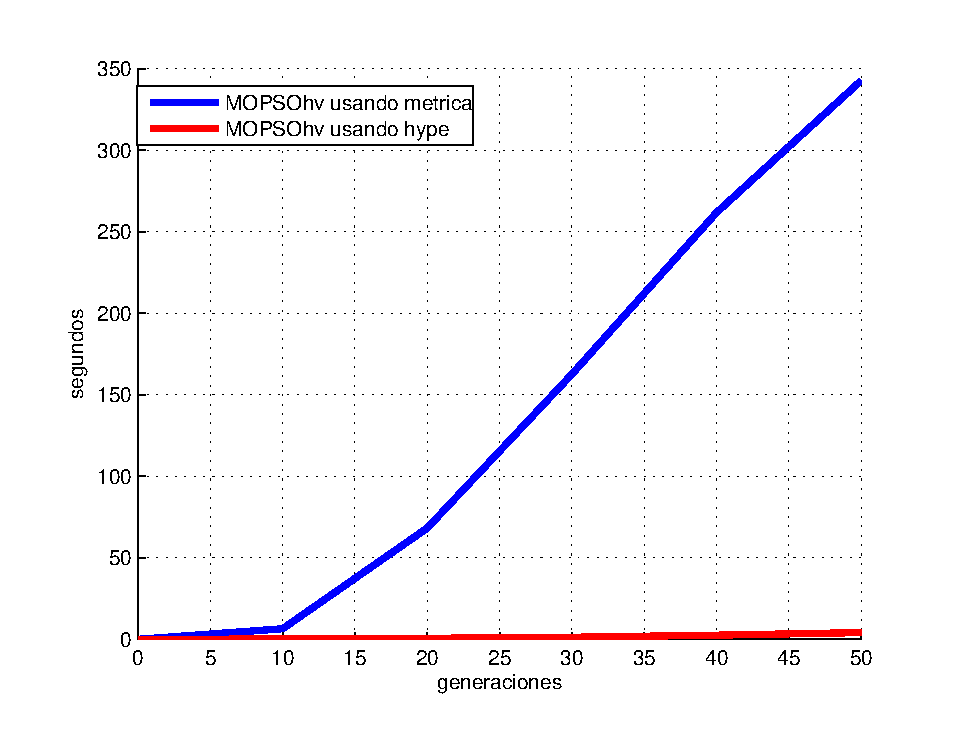
\includegraphics[scale=0.6]{time3.eps}
      \end{center}	
     
      \end{figure}
\end{frame}
% =========================================================================================================
\begin{frame}
	\frametitle{Actualizar $pBest$}	
	\begin{algorithm}[H]
		$nttop = ((tam_A - 1) \cdot r)$\;
		$top = ((tam_A - 1) \cdot p)$\;
		\For { cada part\'icula $i$ hasta $tam_S$}{
	   $j= RandomInt(top+1,nttop)$\;
	   $pBest^t_i = A^t_j$\;
	}
	\Return $pBest^t$\;	
	\caption{Actualizar $pBest$}
	\end{algorithm}
\end{frame}
% =========================================================================================================
\begin{frame}
	\frametitle{Influencia de los modelos de configuraci\'on}	
	\begin{figure}[H]
	\centering
	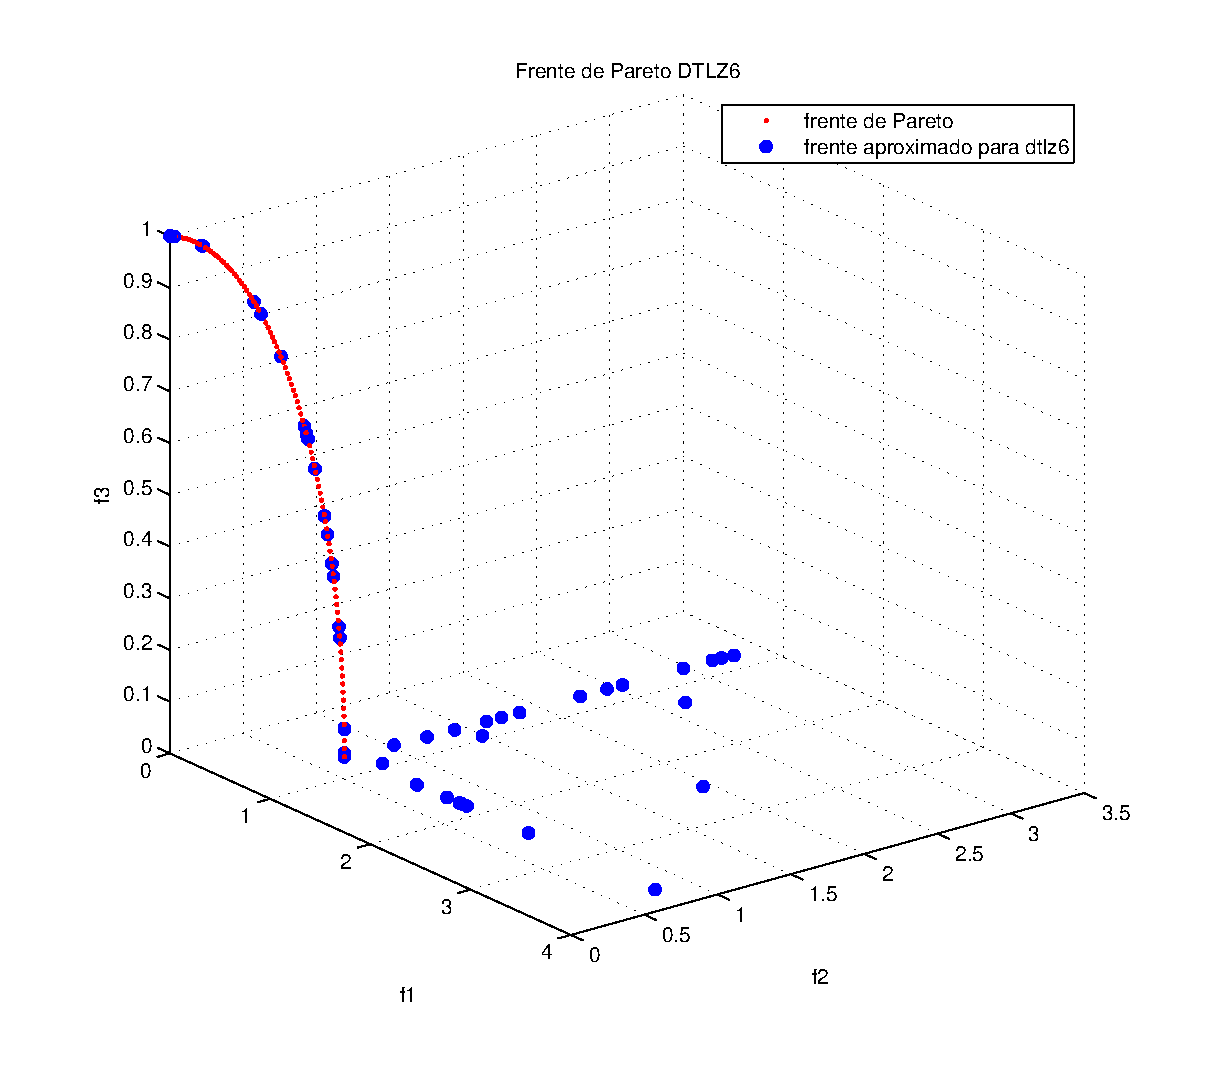
\includegraphics[scale=0.45]{idtlz6.eps}
     
      \end{figure}
\end{frame}

% =========================================================================================================
\begin{frame}
	\frametitle{Influencia de $pBest$}	
	\begin{figure}[H]
	\centering
	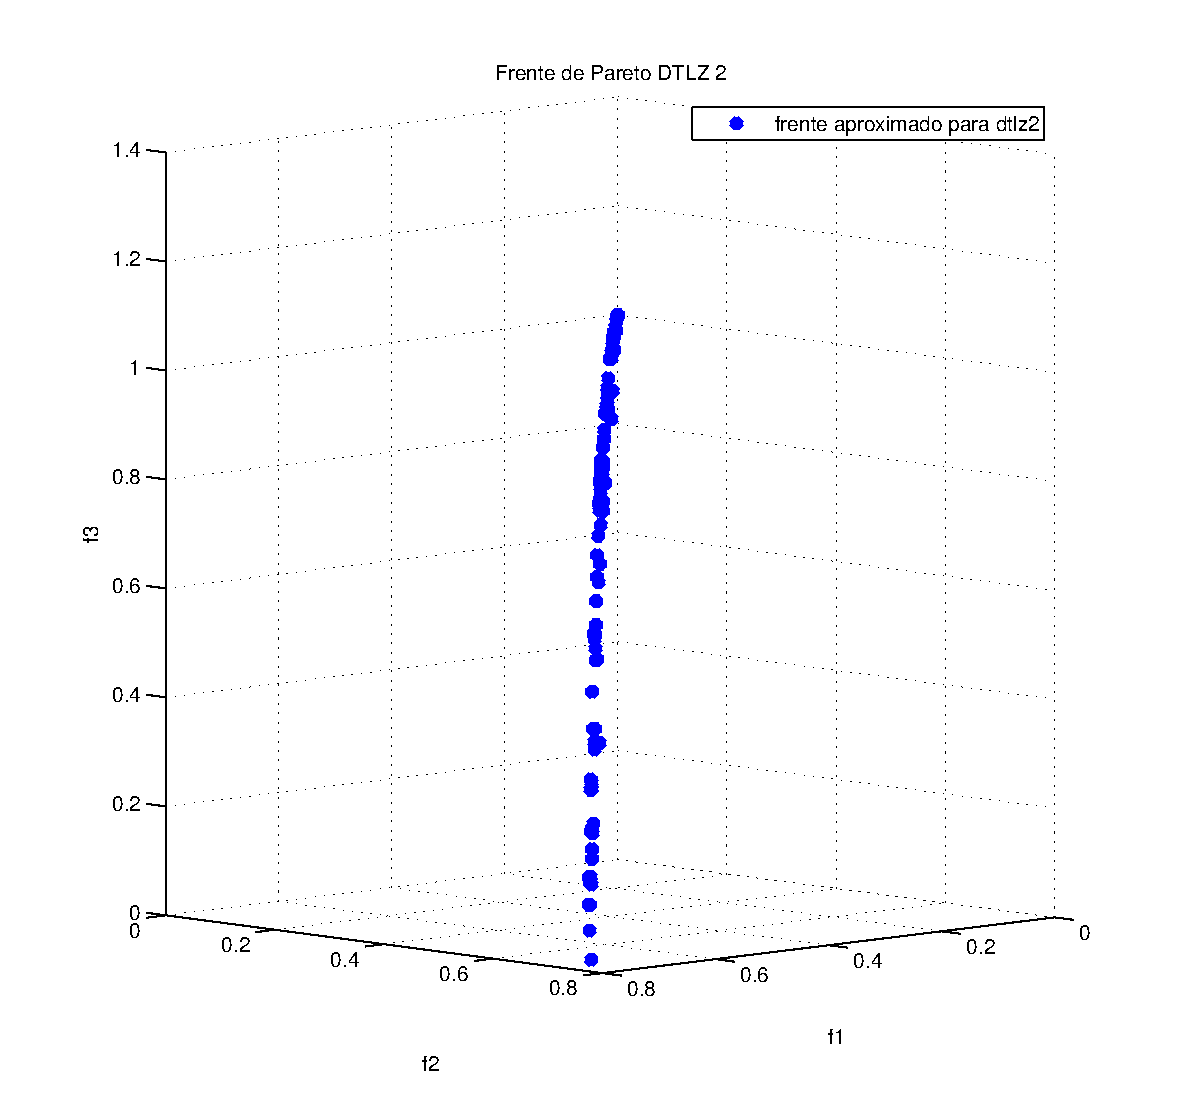
\includegraphics[scale=0.45]{idtlz2.eps}
    
      \end{figure}
\end{frame}
% =========================================================================================================
\begin{frame}
	\frametitle{Operador de turbulencia}	
	 \begin{algorithm}[H]			
			Part\'icula $S_i$ para mutar, $dim$ el n\'umero de dimensiones, $max_{Gen}$ el n\'umero m\'aximo de generaciones,
	      $pMuta$ la probabilidad de mutaci\'on y $t$ la generaci\'on actual\;			
			\If {$flip \left( \left( 1 - t / max_{Gen}  \right)^{5/pMuta} \right) $} {
				$wdim = random(0, dim-1)$\;
				$rango = \left(u_{wdim} - l_{wdim}\right)\cdot \left(1 - t/max_{Gen} \right)^{5/pMuta}$\;
				$ub = S_{i,wdim} + rango$\;
				$lb = S_{i,wdim} + rango$\;
				\If{$lb < l_{wdim}$}{
					$lb = l_{wdim}$\;
					}	  
				\If{$ub > u_{wdim}$}{
					$ub = u_{wdim}$\;
				}
			$S_{i,wdim} = random\left(lb,ub\right)$\;
	}
	\Return Part\'icula $S_i$ mutada\;  
	\caption{Operador de turbulencia}
  \end{algorithm}

\end{frame}
% =========================================================================================================
\begin{frame}
	\frametitle{Influencia del operador de turbulencia}	
	\begin{figure}[H]
	\centering
	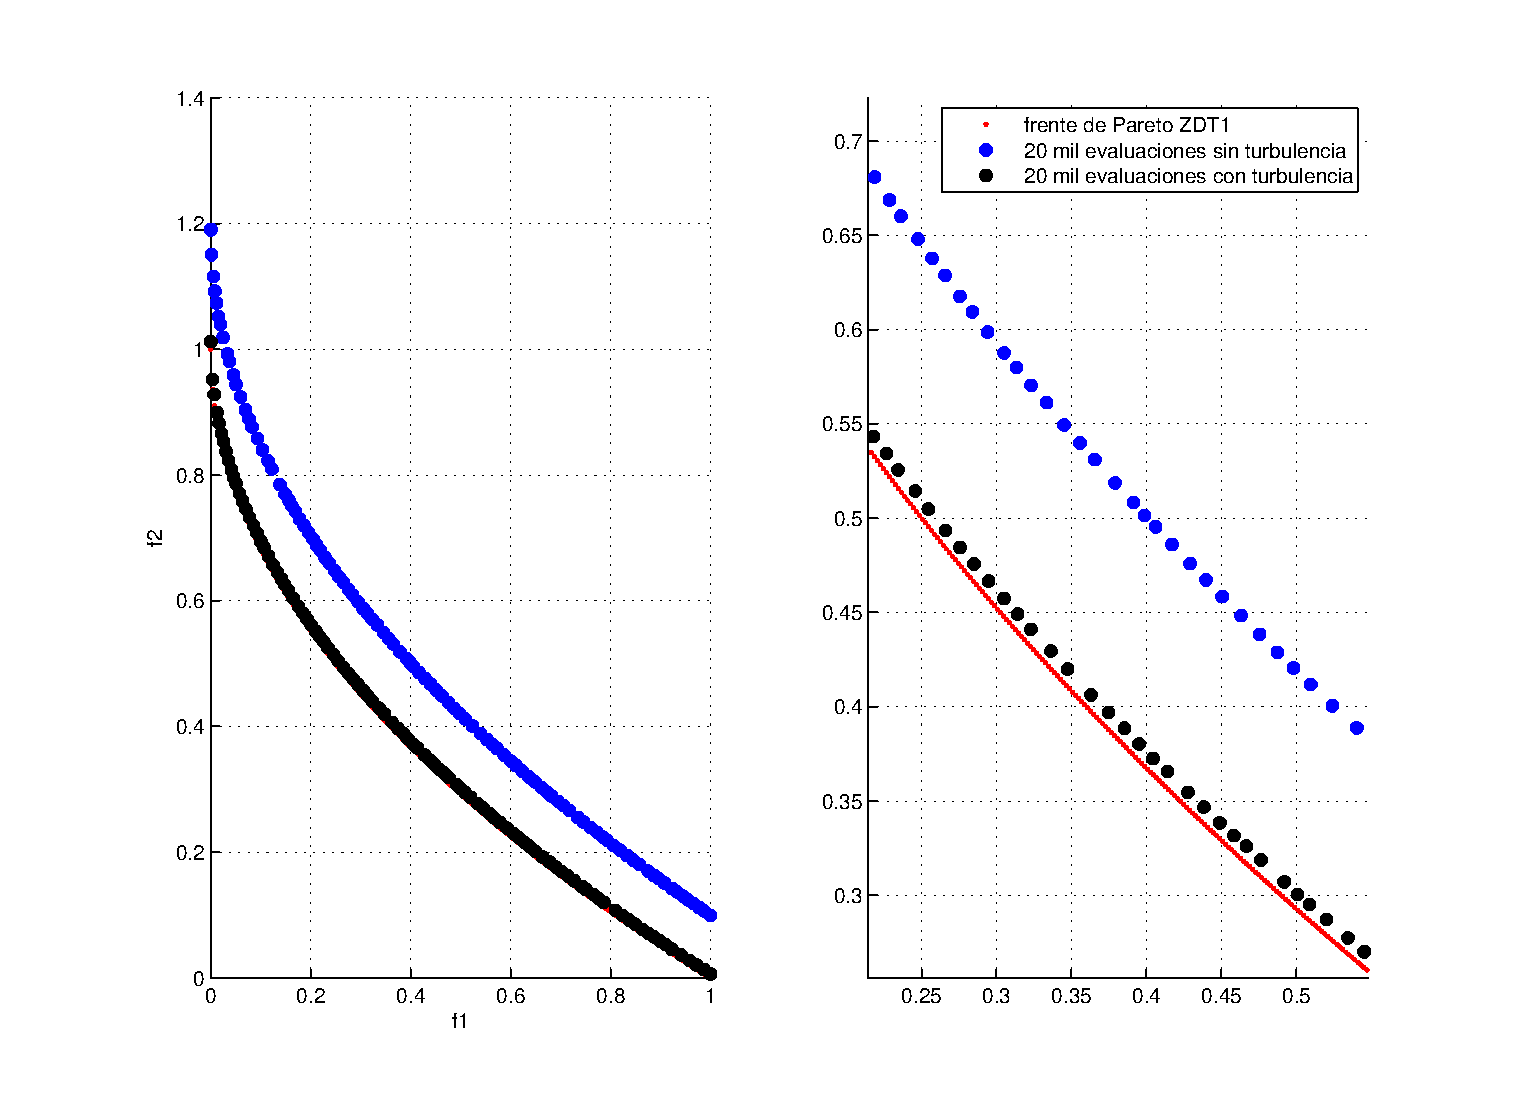
\includegraphics[scale=0.4]{zdt1turbulencia.eps}
      
      \end{figure}
\end{frame}
% =========================================================================================================

\begin{frame}
	\frametitle{Actualizando la posici\'on de las part\'iculas}
		\begin{block}{Factor de inercia}
		\[  
		\vec{v}^{t+1}_{i} = \omega \cdot \vec{v}^t_i + \phi_1 \cdot rnd_1 \cdot \left(\vec{pBest}^t_i - \vec{x}^k_i \right) 
					    + \phi_2 \cdot rnd_2 \cdot \left(\vec{g}^t_i - \vec{x}^t_i \right) 
     \]
  \end{block}
\end{frame}
% =========================================================================================================
\begin{frame}
	\frametitle{Influencia del factor de inercia}	
	\begin{figure}[H]
	\centering
	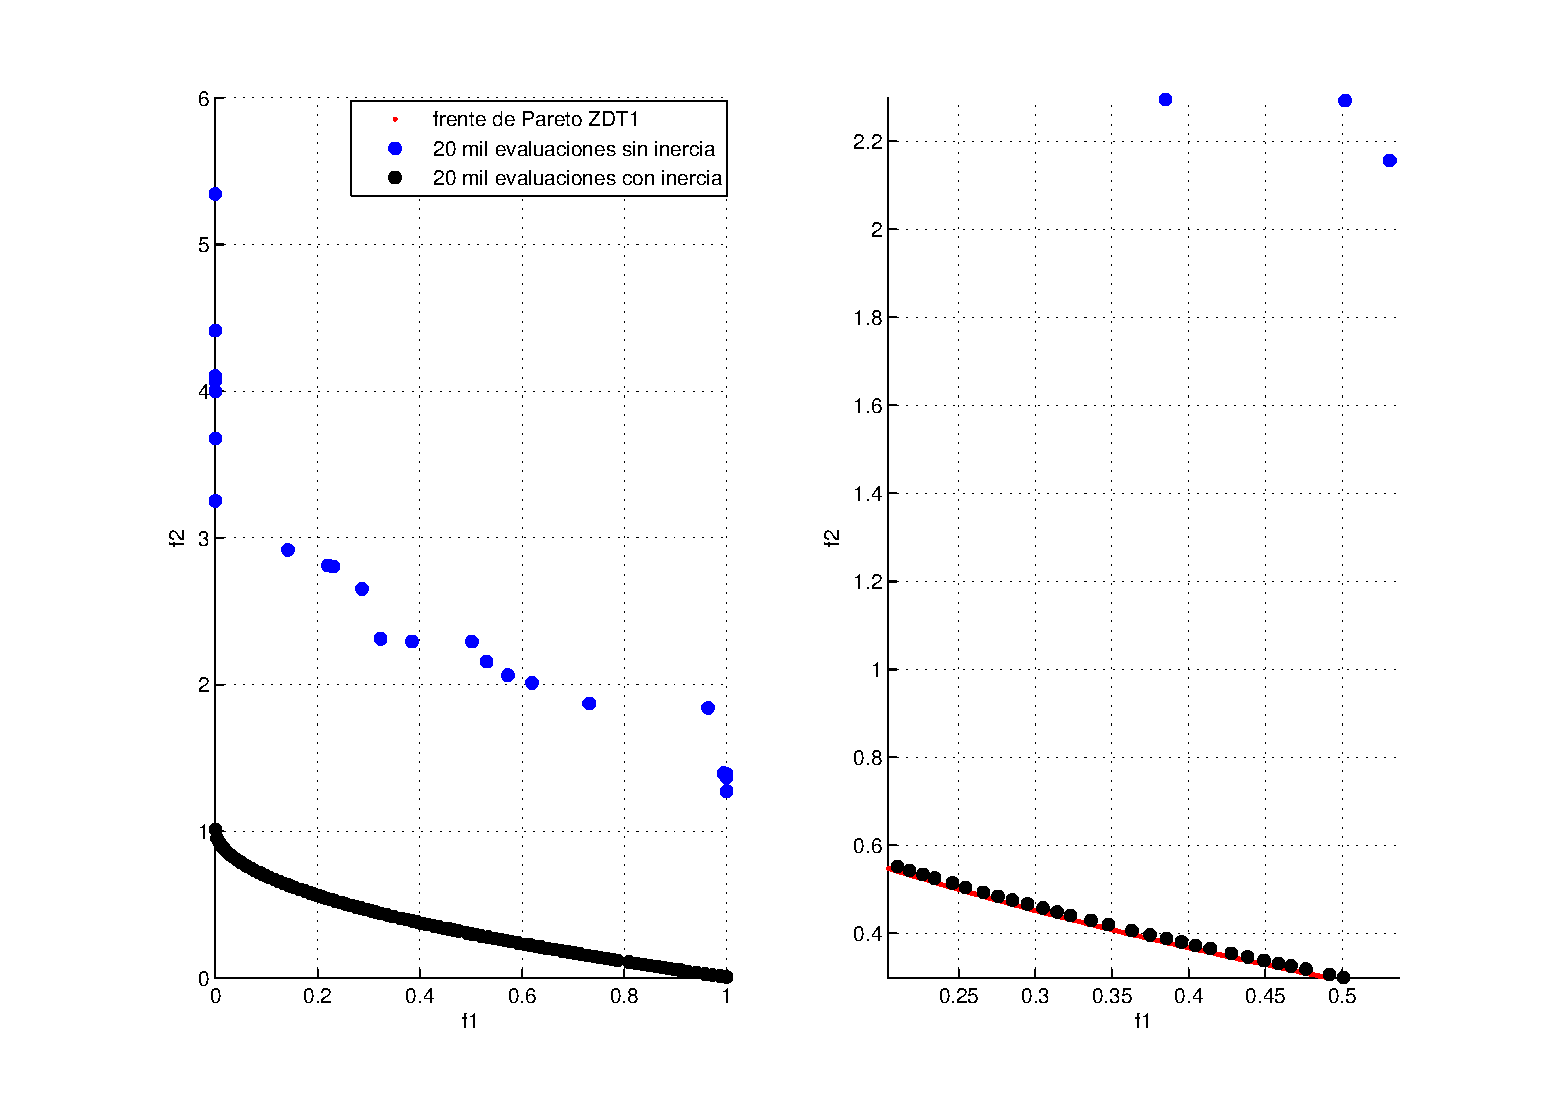
\includegraphics[scale=0.4]{zdt1inercia.eps}
      
      \end{figure}
\end{frame}
% =========================================================================================================

\begin{frame}
\frametitle{¿Por qu\'e de la selecci\'on?}
\begin{figure}[H]
	\centering
	\includegraphics[scale=0.4]{presentacion-4.eps}      
      \end{figure}
  %agregar el boxplot de la metrica
\end{frame}
% =========================================================================================================
\begin{frame}
	
	\begin{figure}[H]
	\centering
	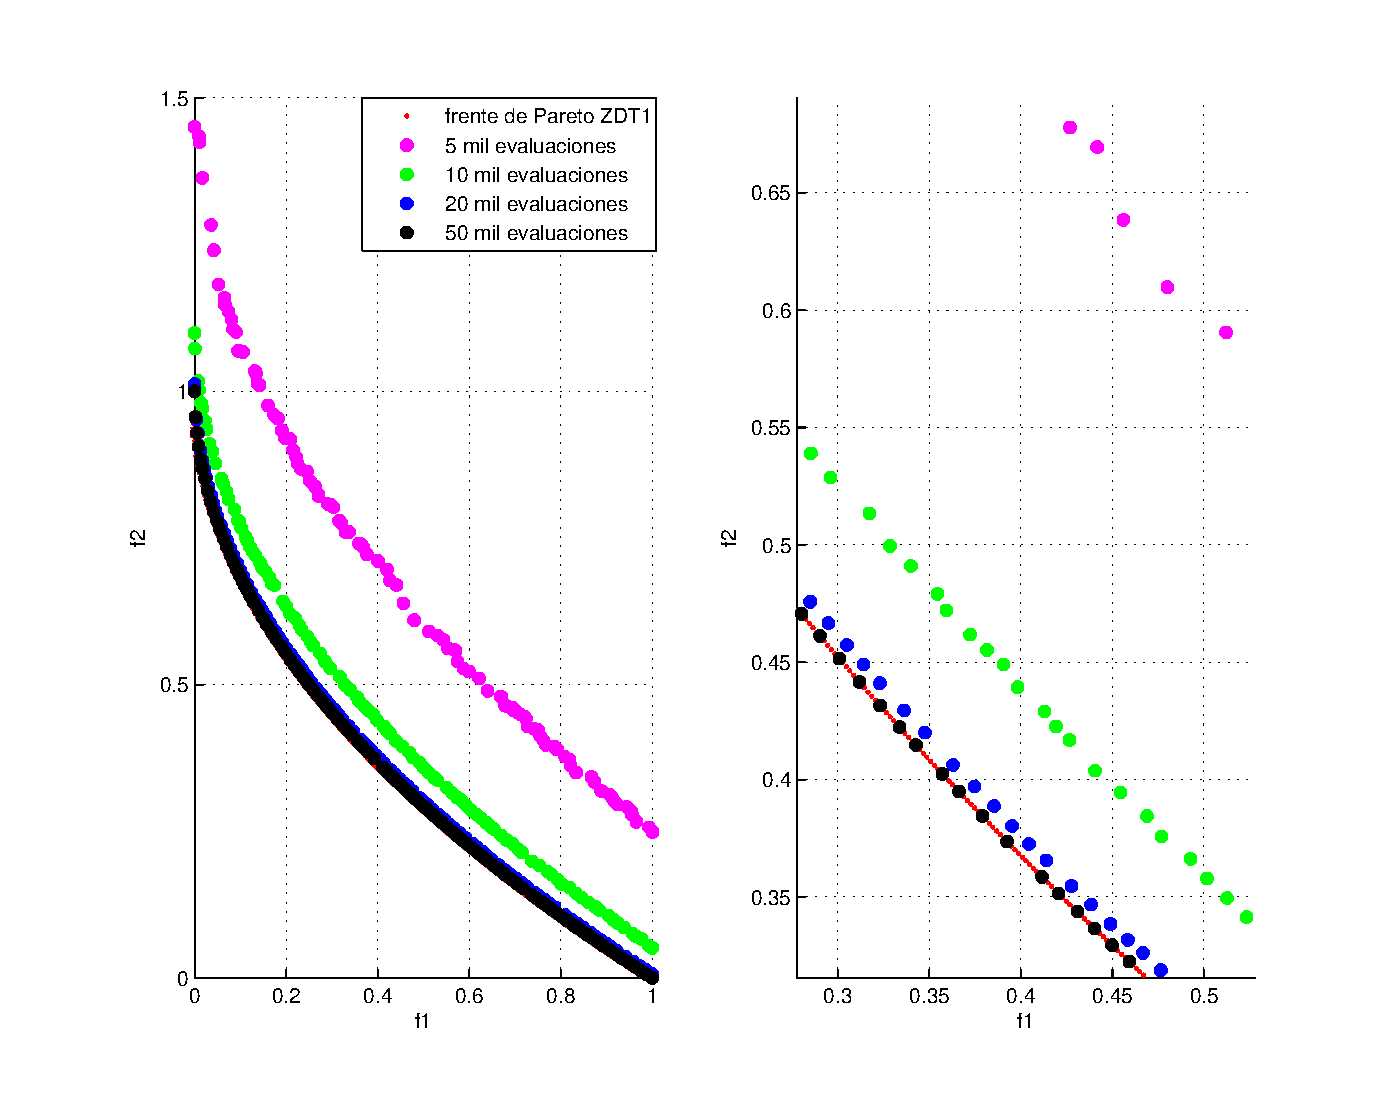
\includegraphics[scale=0.45]{zdt1varios.eps}      
      \end{figure}
\end{frame}

% =========================================================================================================

\section{Experimentos}
\frame{\tableofcontents[currentsection]}
\subsection{Indicadores de Calidad}
% =========================================================================================================
\begin{frame}
	\frametitle{Indicadores de calidad}
	\begin{block}{Hipervolumen}
			Indica el comportamiento de los algoritmos tanto para la convergencia como para el espaciado de las soluciones.
	\end{block}
	\begin{block}{Distancia Generacional Invertida (IGD)}
		Determina cu\'an lejos se encuentra el verdadero frente de Pareto, del frente obtenido por el algoritmo.
		$$
	IGD = \frac{1}{N} \cdot \sqrt{\sum^{N}_{i=1}{d^2_i}},
      $$     
      donde $N$ es la cantidad de puntos del verdadero frente de Pareto, 
			$d_i$ la distancia euclidiana entre cada punto del verdadero frente, al punto m\'as cercano del frente obtenido.       
	\end{block}
\end{frame}
% =========================================================================================================
\begin{frame}
	\frametitle{Indicadores de calidad}
	\begin{block}{Cobertura de conjuntos ($\mathcal{C}$)}
		Determina cuantitativamente cu\'anto un conjunto cubre o domina a otro.
		$$
	      \mathcal{C}\left(A, B \right) = \frac{|\vec{b} \in B; \exists \vec{a} \in A: \vec{a}\preceq \vec{b}|}{|B|}
	  $$
	\end{block}
	\begin{block}{Espaciado}
		 Determina la dispersi\'on de los puntos sobre el frente. Es utilizada para conocer 
	 c\'omo est\'an distribuidas las soluciones a lo largo del frente de Pareto.
		 $$S= \frac{d_f + d_l + \sum^{N-1}_{i=1}{|d_i-d^{'}|}}{d_f + d_l + \left(N -1\right)\cdot d^{'}}$$
  
      donde $N$ es la cantidad de puntos del frente, $d_i$ es la distancia euclidiana entre soluciones consecutivas, 
      $d^{'}$ es el valor medio de todas las distancias y, $d_f$ y $d_l$ son las distancias euclidianas a los extremos 
      del frente de Pareto.
	\end{block}
\end{frame}
% =========================================================================================================
\begin{frame}
	\frametitle{Par\'ametros }
	\begin{block}{MOPSOhv y MOPSOcd}
	Los par\'ametros utilizados para generar las soluciones de los algoritmos MOPSOhv y MOPSOcd:
	
	\begin{table}[H]
  \begin{center}
    \begin{tabular}{|l||c|c|c|}
	\hline
	& \textbf{Generaciones}  & \textbf{Poblaci\'on} & \textbf{Mutaci\'on} \\
	\hline
	\hline
	\textbf{MOPSOhv} & 1200 & 100 &0.5\\ 
	\hline
	\textbf{MOPSOcd} & 1200 & 100 &0.5\\
	\hline
	\end{tabular}
  \end{center}		
	
\end{table}
Se us\'o un factor de inercia $\omega = 0.4$ y constantes sociales $\phi_{1}=\phi_{2}=1$.
 \end{block}
\end{frame}
% =========================================================================================================

\begin{frame}
	\frametitle{Par\'ametros}
		\begin{block}{NSGA-II}
		\begin{table}[H]
  \begin{center}
    \begin{tabular}{|l||c|c}
	\hline
	Generaciones  & 1200 \\ 
	\hline
	Poblaci\'on & 100 \\ 
	\hline
	Cruza & 0.9 \\
	\hline
	Mutaci\'on & $\frac{1}{\vec{x}}$ \\
	\hline
  \end{tabular}

\end{center}
\end{table}
		\end{block}
		
		\begin{block}{SMS-EMOA}
		\begin{table}[H]
	\begin{center}
		\begin{tabular}{|l||c|c}
			\hline
			Generaciones  & 1200 \\ 
			\hline
			Poblaci\'on & 100 \\ 
			\hline
			$\eta_c = \eta_m$ & 20 \\ 
			\hline
			Mutaci\'on & $\frac{1}{\vec{x}}$\\ 
			\hline			
		\end{tabular}
	\end{center}
\end{table}
		\end{block}
\end{frame}
% =========================================================================================================

\subsection{Resultados}
\begin{frame}
	\frametitle{ZDT1, ZDT2 Y ZDT3}	
	\begin{block}{Conforme a estos resultados se tiene una jerarqu\'ia en orden descendente en t\'erminos de convergencia en estos primeros tres 
  problemas}
\begin{enumerate}
  \item SMS-EMOA
  \item MOPSOhv
  \item NSGA-II
  \item MOPSOcd
\end{enumerate}
\end{block}
\end{frame}
% =========================================================================================================
\begin{frame}
	\frametitle{ZDT4 y ZDT6}	
	\begin{block}{Conforme a estos resultados se tiene una jerarqu\'ia en orden descendente en t\'erminos de convergencia en estos dos 
  problemas}
  
  \begin{enumerate}
  \item NSGA-II
  \item SMS-EMOA
  \item MOPSOhv
  \item MOPSOcd	
\end{enumerate}
\end{block}
\end{frame}
% =========================================================================================================
\begin{frame}
	\frametitle{ZDT4}	
	\begin{figure}
      \begin{center}
	  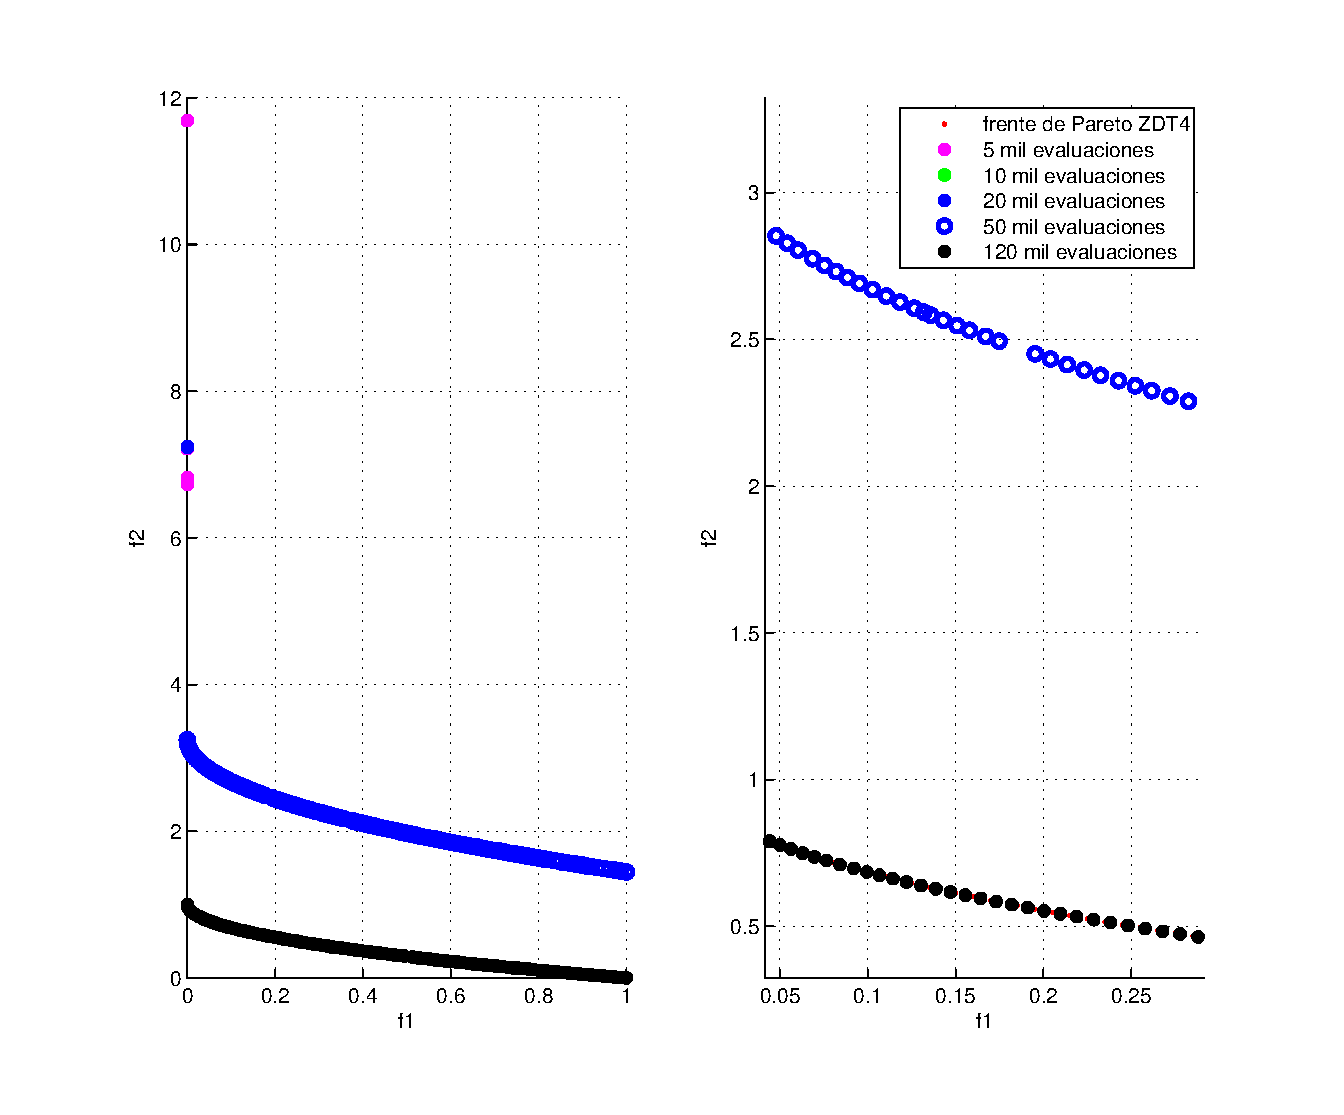
\includegraphics[scale=0.45]{fontzdt4.eps}
      \end{center}      
      \end{figure}
\end{frame}

% =========================================================================================================
\begin{frame}
	\frametitle{DTLZ1, DTLZ3 Y DTLZ4}
\begin{block}{Conforme a estos resultados se tiene una jerarqu\'ia en orden descendente en t\'erminos de convergencia en estos tres 
  problemas}

\begin{enumerate}
  \item NSGA-II
  \item SMS-EMOA
  \item MOPSOhv
  \item MOPSOcd
\end{enumerate}
\end{block}
\end{frame}
% =========================================================================================================
\begin{frame}
	\frametitle{DTLZ2, DTLZ4, DTLZ6 Y DTLZ7}
	\begin{block}{ Conforme a estos resultados se tiene una jerarqu\'ia general en orden descendente en t\'erminos de convergencia para  
 DTLZ4, DTLZ5 y DTLZ7:}

\begin{enumerate}
  \item  NSGA-II
  \item SMS-EMOA
  \item MOPSOhv
  \item MOPSOcd
\end{enumerate}
\end{block}
\end{frame}
% =========================================================================================================
\begin{frame}
	\frametitle{DTLZ2}
	\begin{figure}
      \begin{center}
	  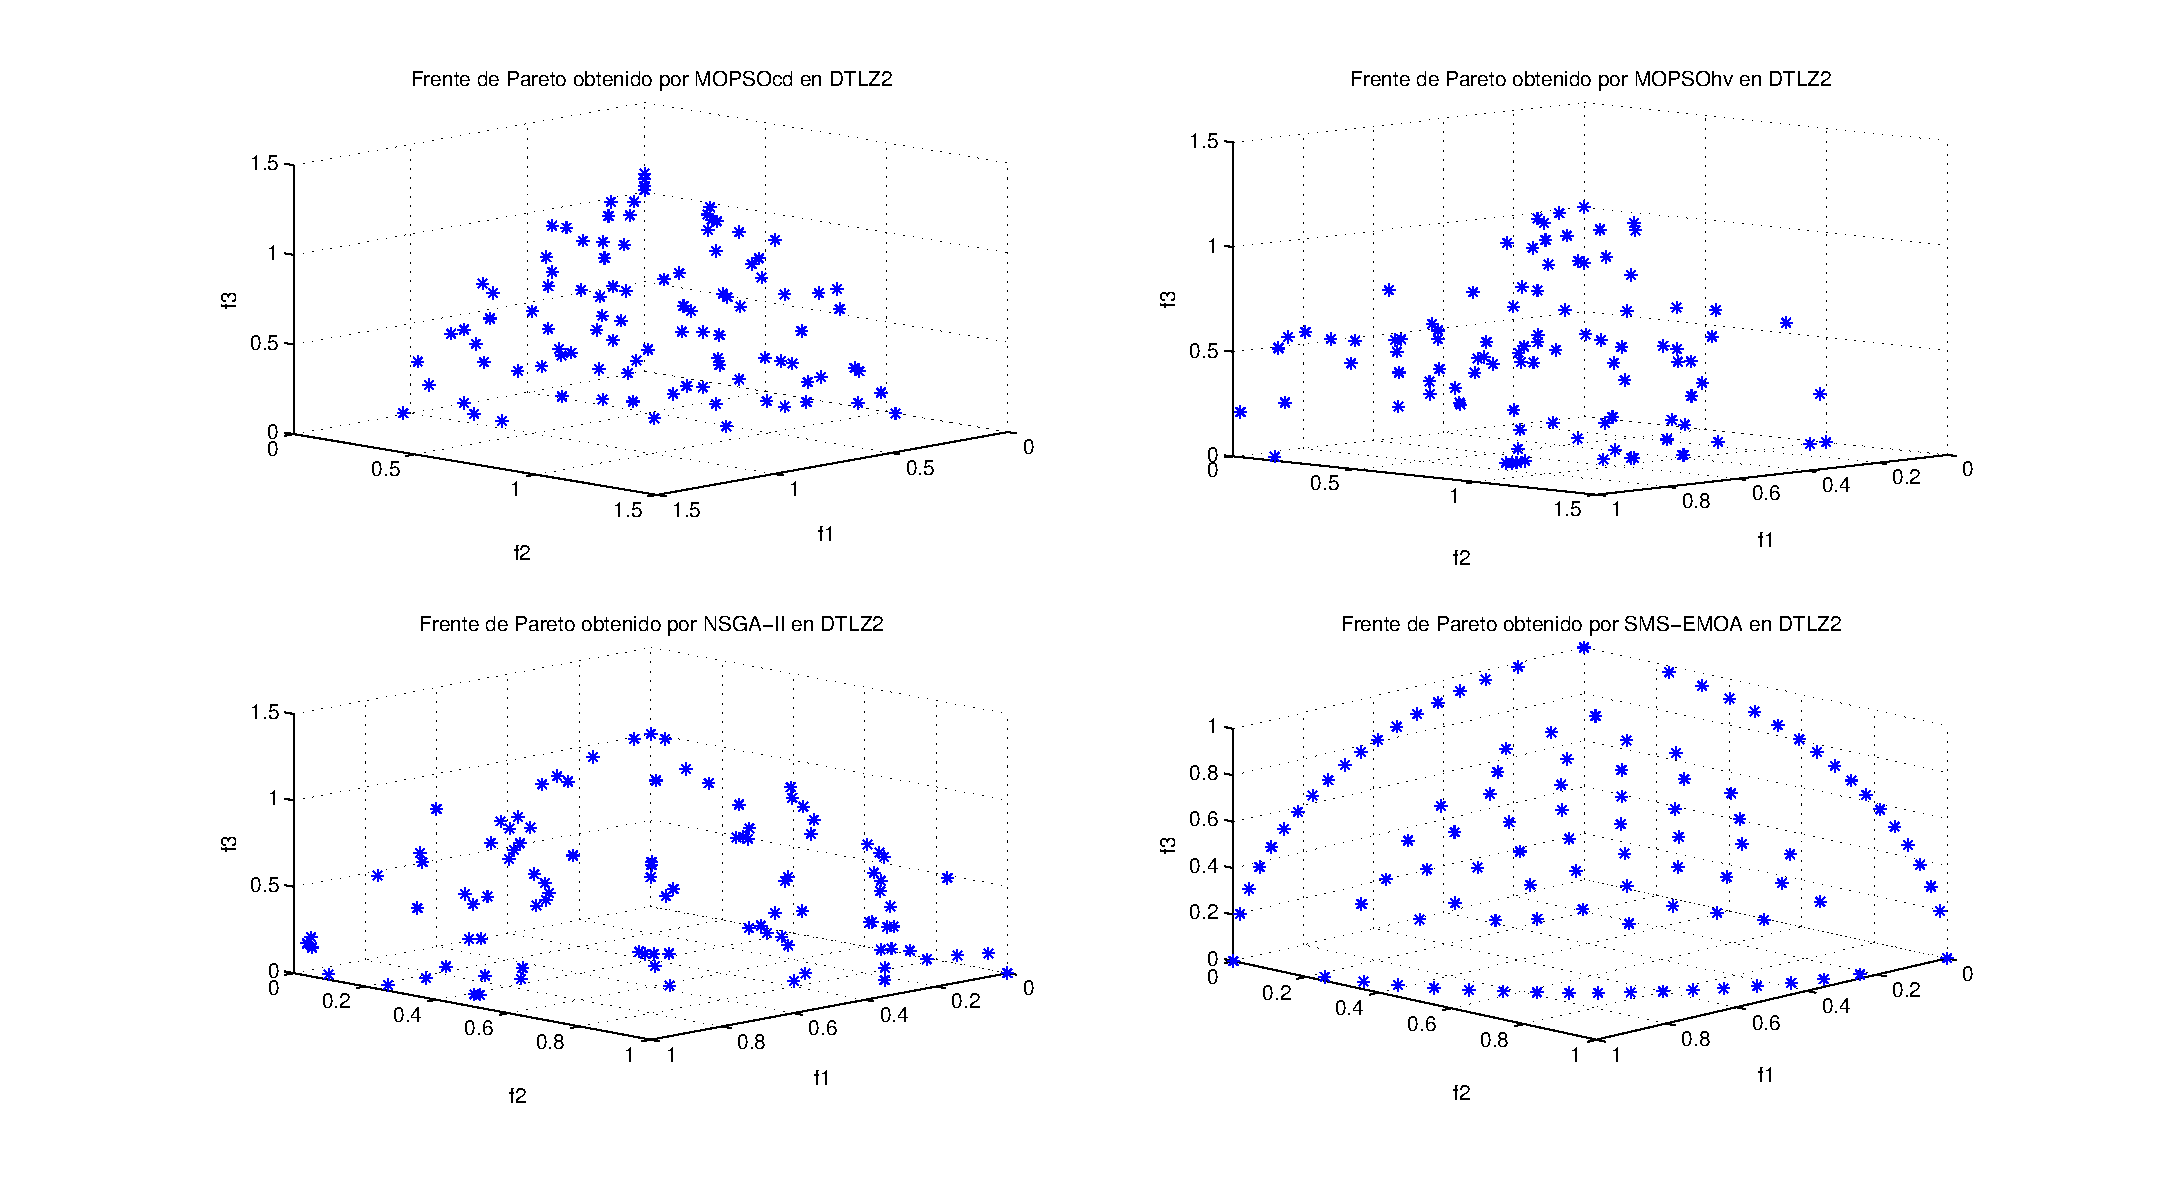
\includegraphics[scale=0.3]{rdtlz2r.eps}
      \end{center}      
      \end{figure}
\end{frame}
% =========================================================================================================
\begin{frame}
	\frametitle{DTLZ4}
	\begin{figure}
      \begin{center}
	  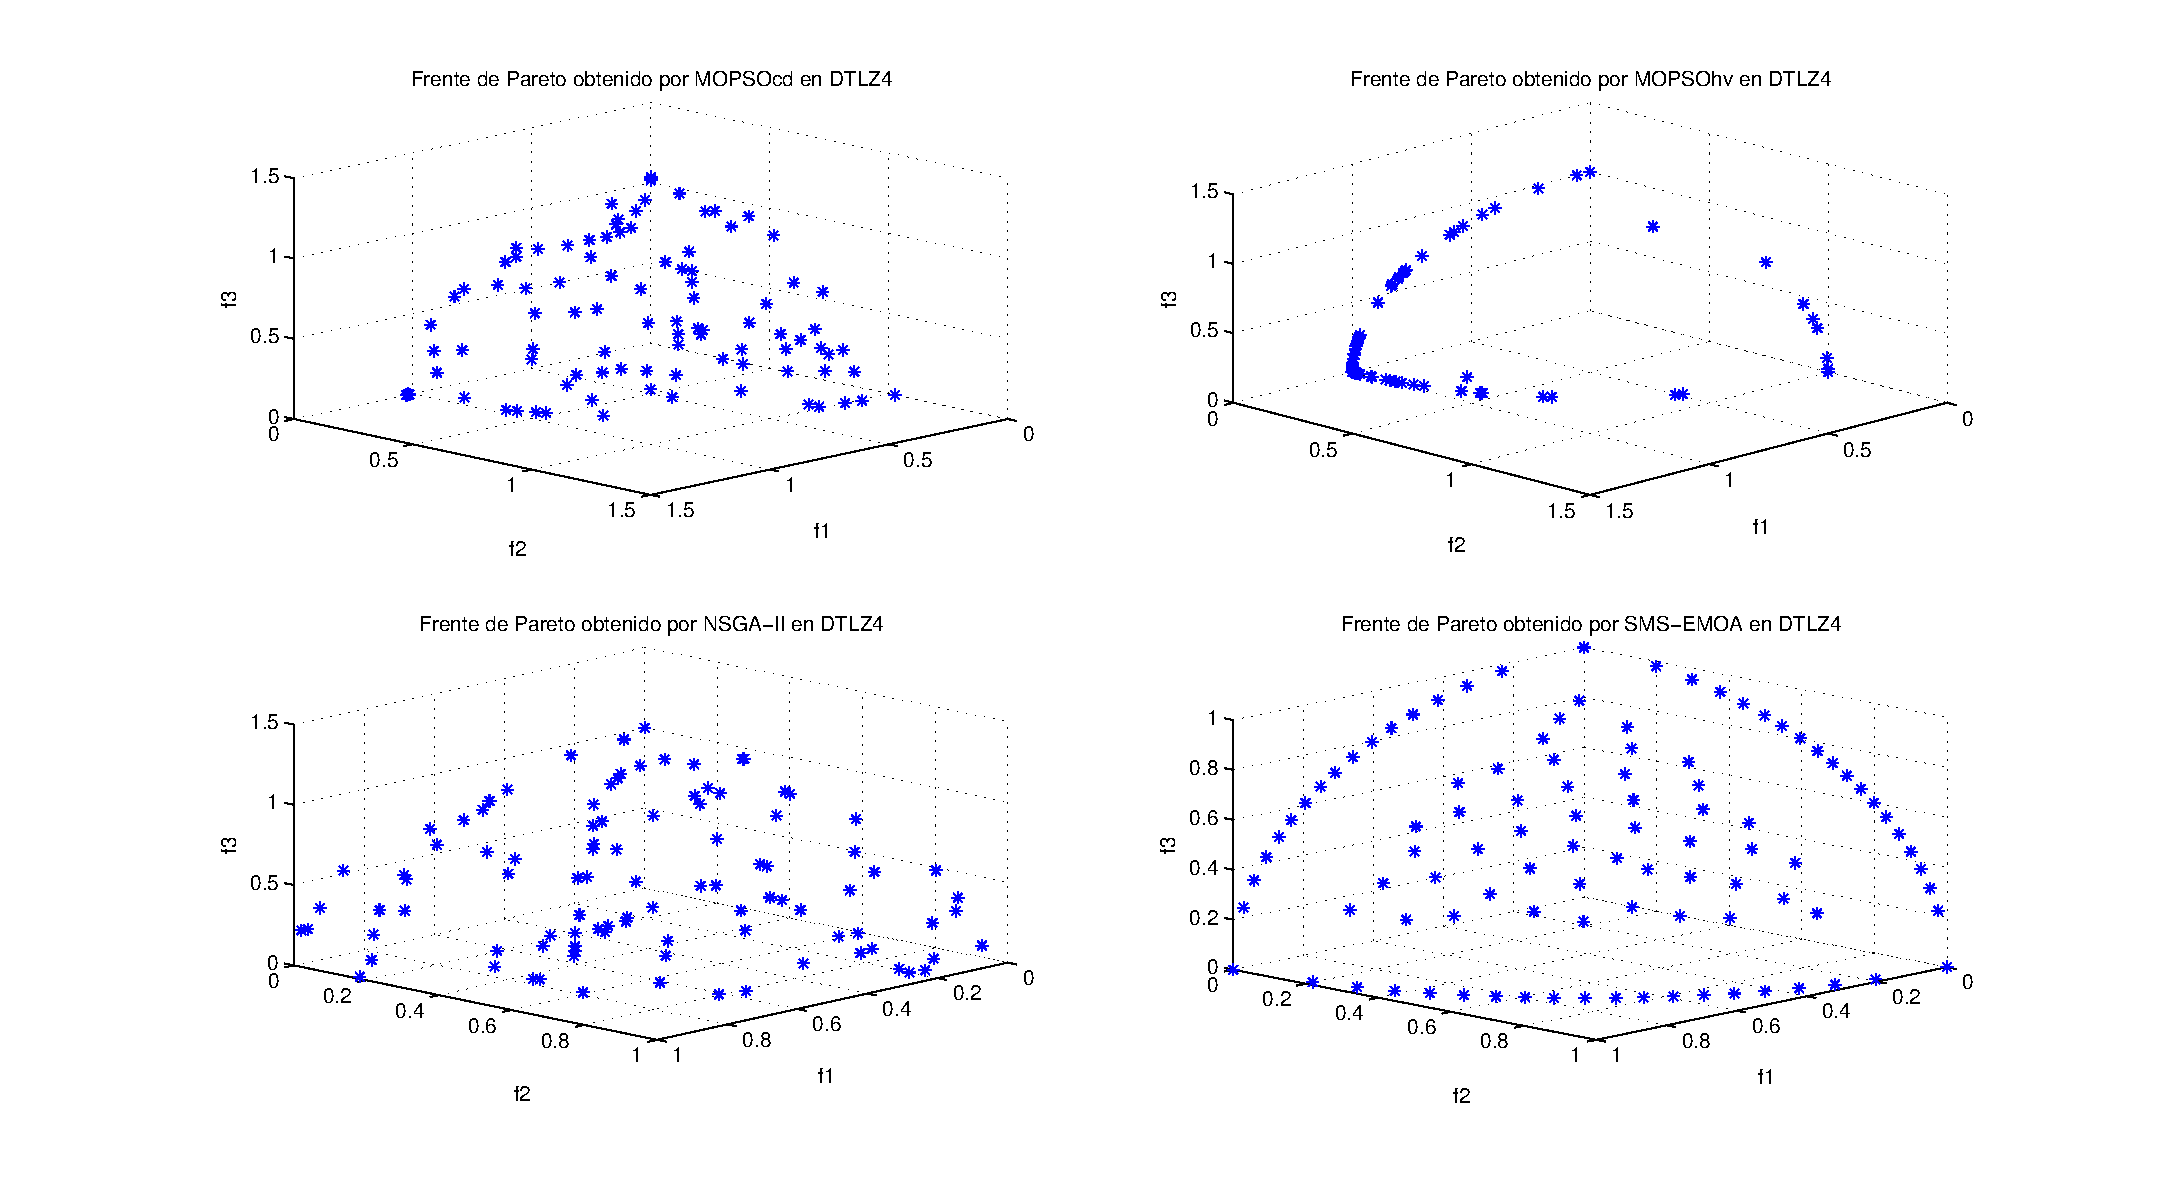
\includegraphics[scale=0.3]{rdtlz4r.eps}
      \end{center}
   \end{figure}
\end{frame}
% =========================================================================================================
\begin{frame}
	\frametitle{DTLZ7}
	\begin{figure}
      \begin{center}
	  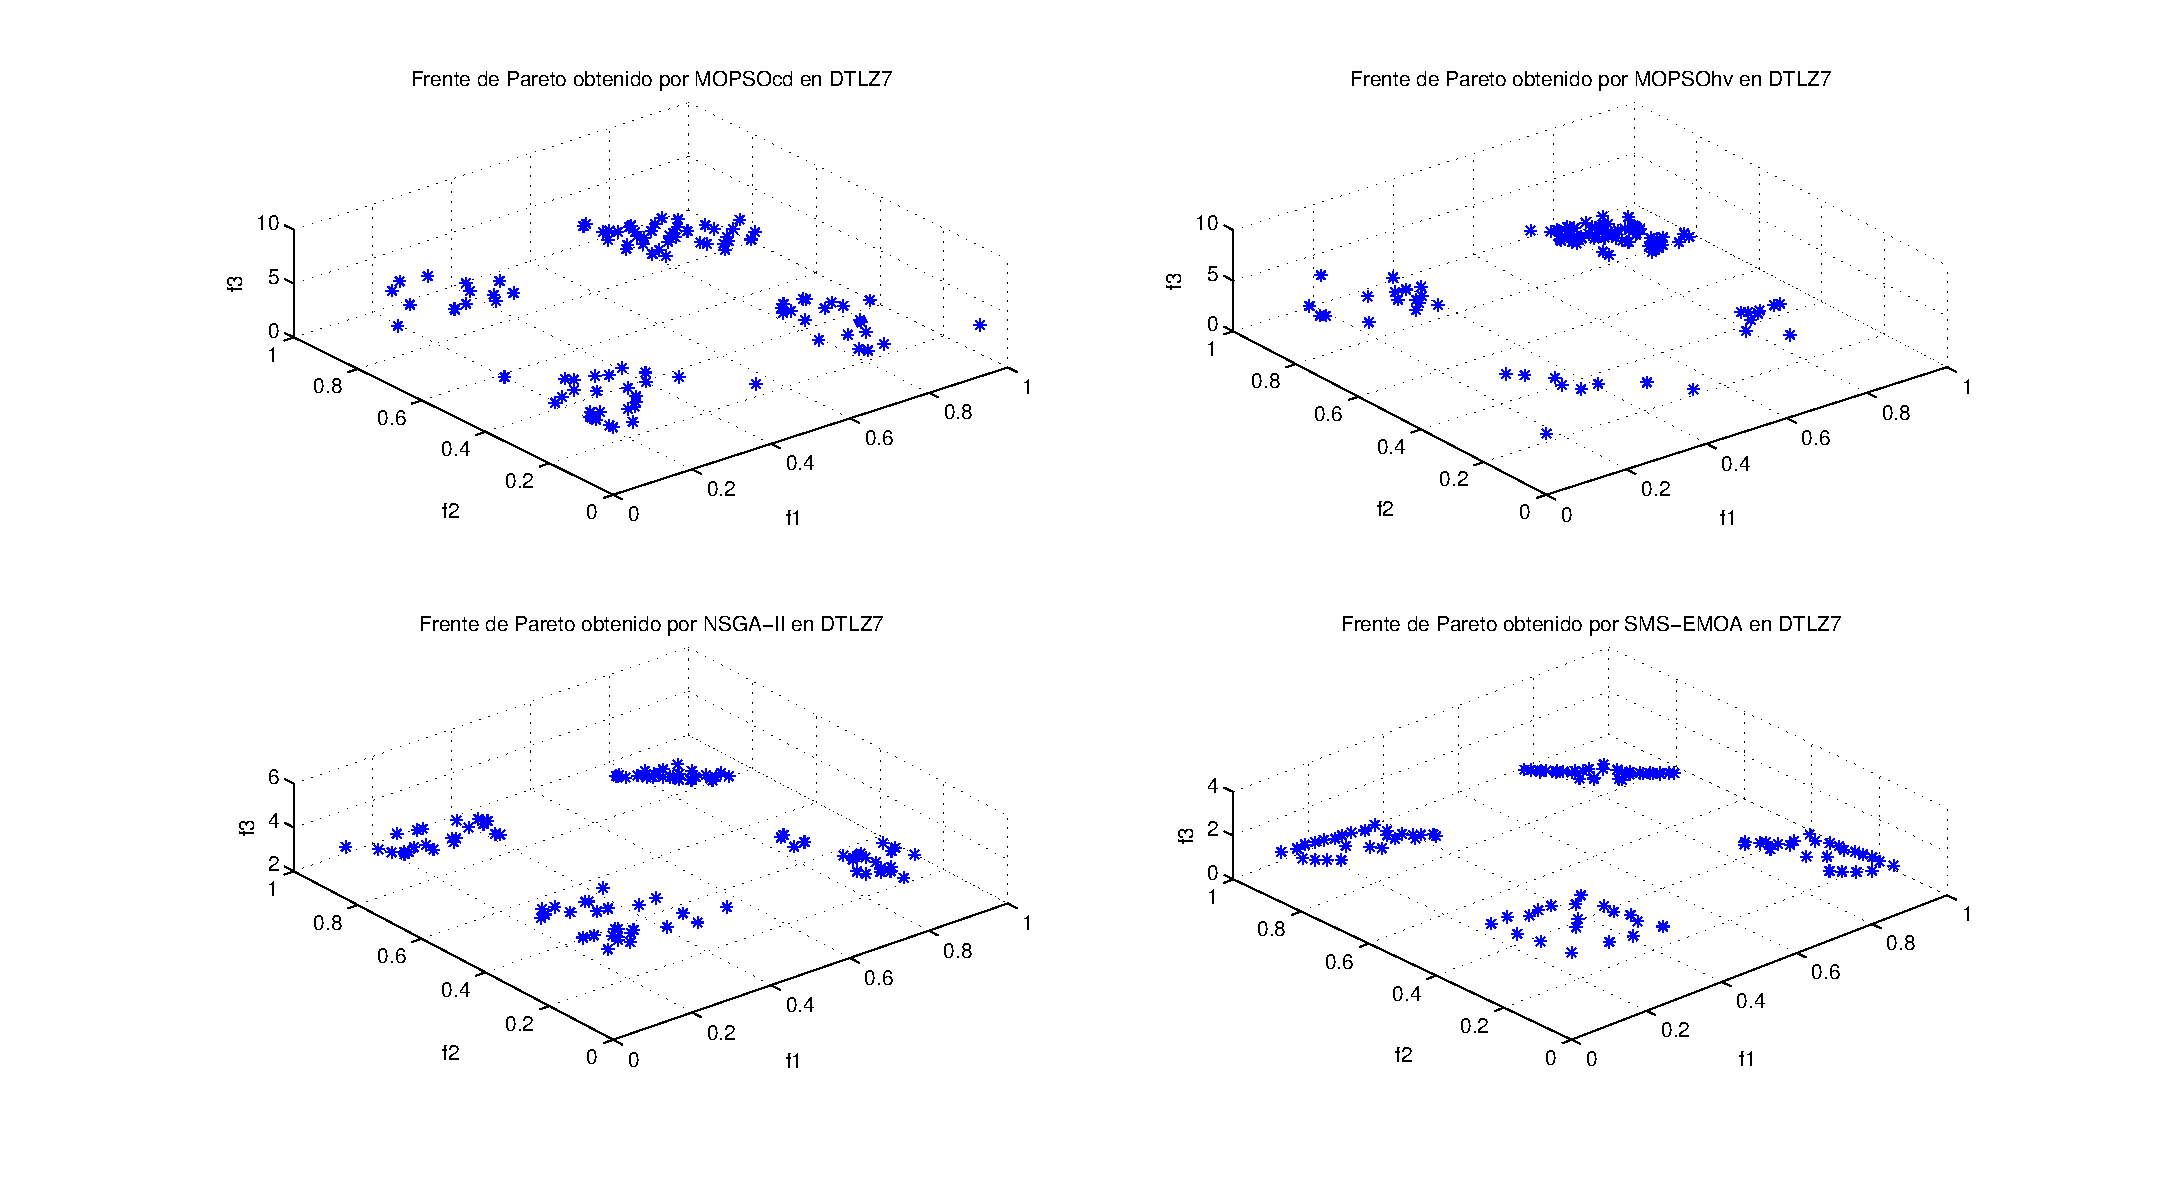
\includegraphics[scale=0.3]{rdtlz7r.eps}
      \end{center}
	    \end{figure}
\end{frame}
% =========================================================================================================
\begin{frame}
\frametitle{Pruebas de escalabilidad (espaciado)} 
 \begin{figure}
      \begin{center}
	  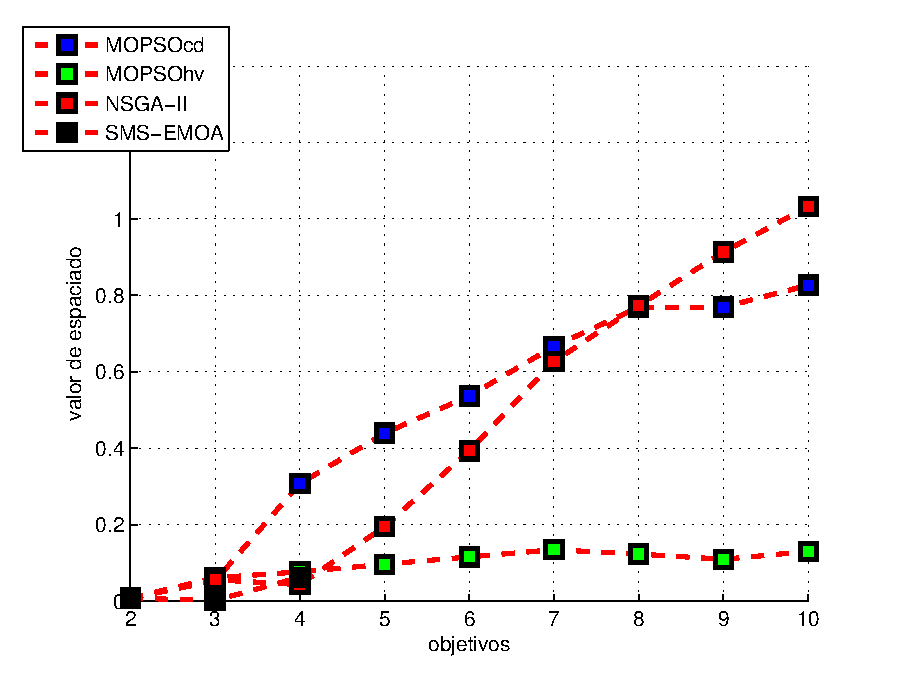
\includegraphics[scale=.7]{espaciadoEscala.eps}
      \end{center}
  \end{figure}
\end{frame}
% =========================================================================================================
\begin{frame}
\frametitle{Pruebas de escalabilidad (hipervolumen)} 
 \begin{figure}
      \begin{center}
	  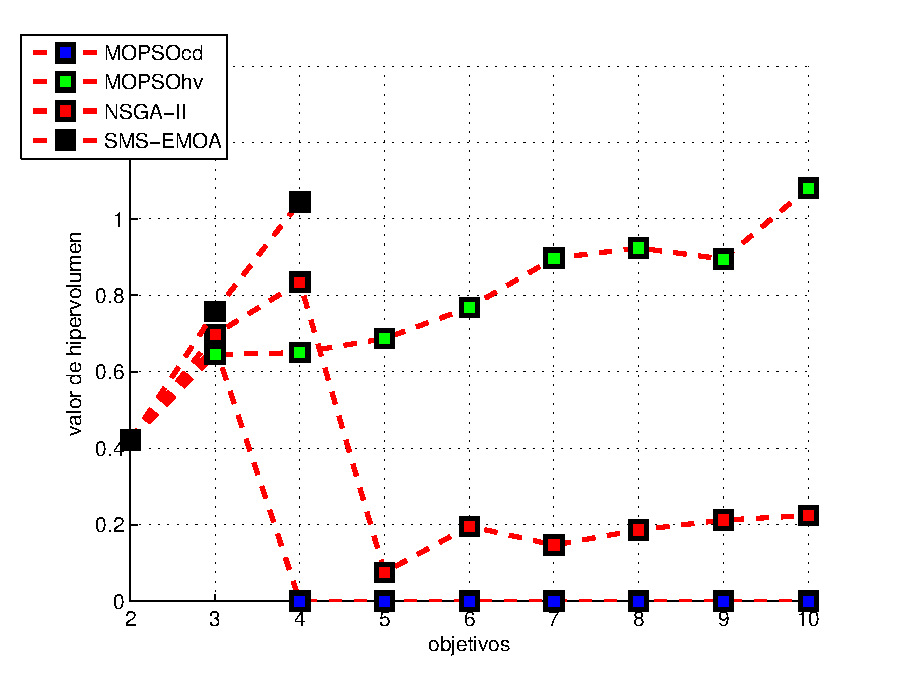
\includegraphics[scale=.7]{hipervolumenEscala.eps}
      \end{center}
  \end{figure}
\end{frame}
% =========================================================================================================
\begin{frame}
\frametitle{Pruebas de escalabilidad (tiempo)} 
 \begin{figure}
      \begin{center}
	  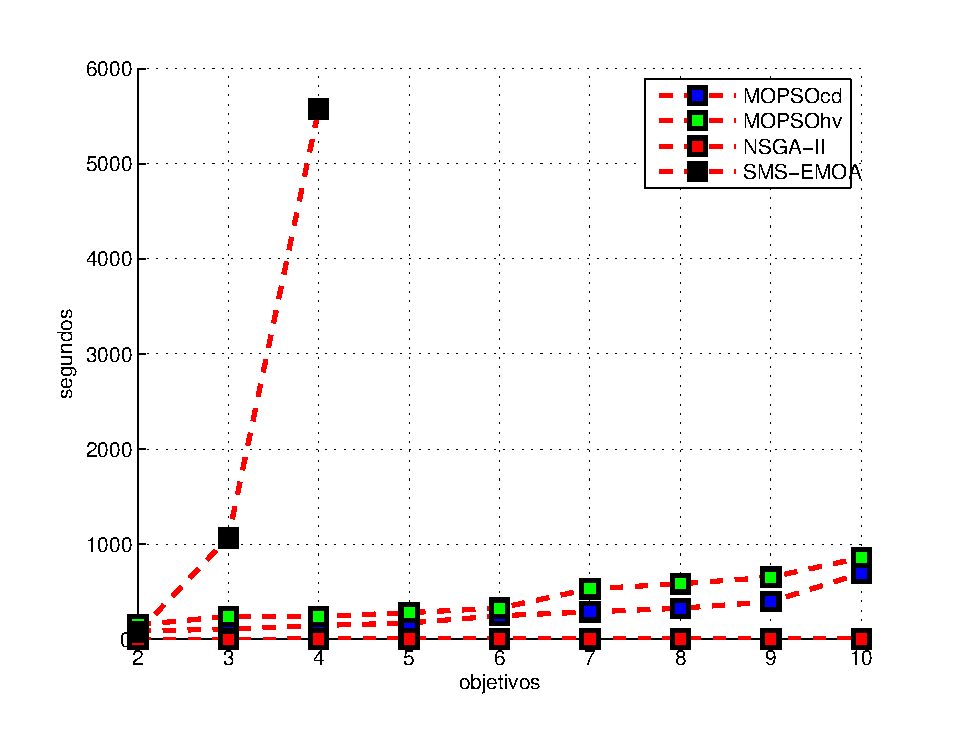
\includegraphics[scale=.6]{tiempoEscala.eps}
      \end{center}
  \end{figure}
\end{frame}

% =========================================================================================================
\begin{frame}
\frametitle{¿Por qu\'e escala?}
\begin{figure}
      \begin{center}
	  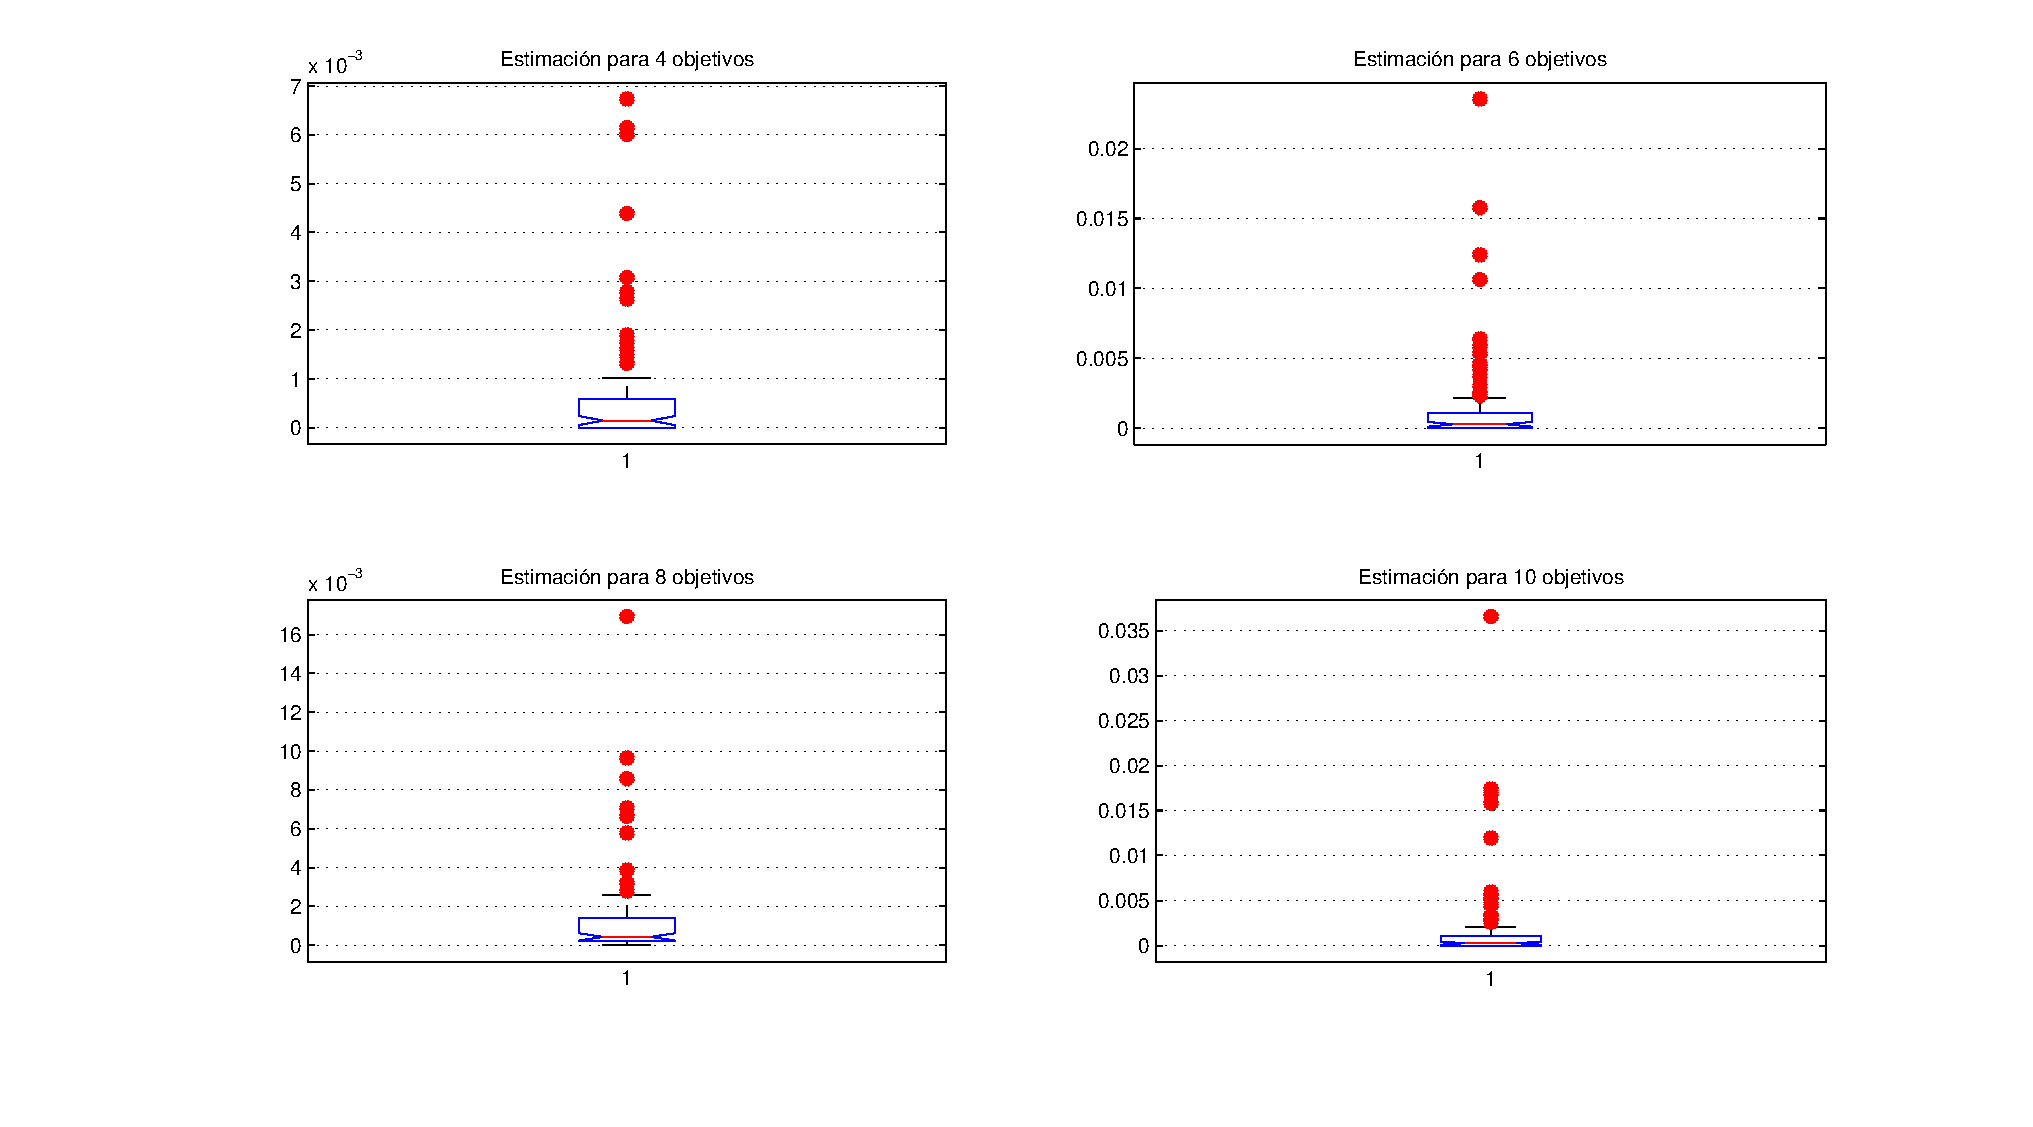
\includegraphics[scale=.35]{pqescala.eps}
      \end{center}
  \end{figure}
\end{frame}
% =========================================================================================================
\section{Conclusiones y Trabajo Futuro}
\frame{\tableofcontents[currentsection]}
\begin{frame}
	\frametitle{Conclusiones}
	\begin{block}{A partir de los experimentos realizados se desprenden las siguientes conclusiones:}
	\begin{itemize}
   
  \item La forma de seleccionar el conjunto de part\'iculas que influyen en el entorno social mejora 
  la b\'usqueda de nuevas soluciones. 
  
  \item El uso de un algoritmo que estima las contribuciones al hipervolumen permite aumentar el n\'umero de generaciones 
  del algoritmo y el n\'umero de objetivos del problema.
  
  \item Debido a que se utiliza una aproximaci\'on de la contribuci\'on al hipervolumen, se decidi\'o utilizar un operador de 
  turbulencia para evitar quedar atrapado en frentes de Pareto locales.
    
  \item Muestra tener buenos resultados en la mayor\'ia de los problemas (2 y 3 objetivos).
  
  \item Mantiene un buen desempe\~no al aumentar el n\'umero de objetivos del problema, manteniendo un costo computacional 
  razonable.
  \end{itemize}
	\end{block}
\end{frame}
	% =========================================================================================================


\begin{frame}
	\frametitle{Trabajo futuro}	
	
\begin{block}{En particular se podr\'ian realizar las siguientes extensiones a nuestro algoritmo:}
  
  \begin{itemize}
		\item Utilizar modelos de configuraci\'on diferentes al modelo completo.
		\item Utilizar otros apectos avanzados que pueden acelerar la convergencia del algoritmo.  
		\item Seleccionar a los gu\'ias locales de otra manera, de tal forma, que afecten la parte cognitiva del algoritmo permitiendo
 generar nuevas soluciones.
		\item Seleccionar un mejor estimador de densidad para hacer el reemplazo de los soluciones no dominadas en la poblaci\'on secundaria.
	\end{itemize}
	\end{block}
\end{frame}
% =========================================================================================================
\begin{frame}
	\frametitle{¿Preguntas?}
	\begin{center} {\huge Gracias por su atenci\'on}
	\end{center}

\end{frame}
% =========================================================================================================
\end{document}
